% $Id: template.tex 11 2007-04-03 22:25:53Z jpeltier $

%\documentclass{vgtc}                          % final (conference style)
\documentclass[review]{vgtc}                 % review
%\documentclass[widereview]{vgtc}             % wide-spaced review
%\documentclass[preprint]{vgtc}               % preprint
%\documentclass[electronic]{vgtc}             % electronic version

%% Uncomment one of the lines above depending on where your paper is
%% in the conference process. ``review'' and ``widereview'' are for review
%% submission, ``preprint'' is for pre-publication, and the final version
%% doesn't use a specific qualifier. Further, ``electronic'' includes
%% hyperreferences for more convenient online viewing.

%% Please use one of the ``review'' options in combination with the
%% assigned online id (see below) ONLY if your paper uses a double blind
%% review process. Some conferences, like IEEE Vis and InfoVis, have NOTy
%% in the past.

%% Figures should be in CMYK or Grey scale format, otherwise, colour 
%% shifting may occur during the printing process.

%% These three lines bring in essential packages: ``mathptmx'' for Type 1 
%% typefaces, ``graphicx'' for inclusion of EPS figures. and ``times''
%% for proper handling of the times font family.

\usepackage{mathptmx}
\usepackage{graphicx}
\usepackage{times,color,ifpdf}

%% We encourage the use of mathptmx for consistent usage of times font
%% throughout the proceedings. However, if you encounter conflicts
%% with other math-related packages, you may want to disable it.

%% If you are submitting a paper to a conference for review with a double
%% blind reviewing process, please replace the value ``0'' below with your
%% OnlineID. Otherwise, you may safely leave it at ``0''.
\onlineid{109}

%% declare the category of your paper, only shown in review mode
\vgtccategory{Research}

%% allow for this line if you want the electronic option to work properly
\vgtcinsertpkg

%% In preprint mode you may define your own headline.
%\preprinttext{To appear in an IEEE VGTC sponsored conference.}

%% Paper title.

\title{ARmy: Multi-User Interaction in a Spatially Augmented Reality Game}

%% This is how authors are specified in the conference style

%% Author and Affiliation (single author).
%%\author{Roy G. Biv\thanks{e-mail: roy.g.biv@aol.com}}
%%\affiliation{\scriptsize Allied Widgets Research}

%% Author and Affiliation (multiple authors with single affiliations).
%%\author{Roy G. Biv\thanks{e-mail: roy.g.biv@aol.com} %
%%\and Ed Grimley\thanks{e-mail:ed.grimley@aol.com} %
%%\and Martha Stewart\thanks{e-mail:martha.stewart@marthastewart.com}}
%%\affiliation{\scriptsize Martha Stewart Enterprises \\ Microsoft Research}

%% Author and Affiliation (multiple authors with multiple affiliations)

%\author{Andrew Dolce\thanks{e-mail: dolce@somegameplace.com}\\ %
%        \scriptsize Gradient Studios \\
%        \scriptsize Rensselaer Polytechnic Institute
%\and Joshua D. Nasman\thanks{e-mail:nasmaj@cs.rpi.edu}\\ %
%     \scriptsize Rensselaer Polytechnic Institute %
%\and Barbara Cutler\thanks{e-mail:cutler@cs.rpi.edu}\\ %
%     \scriptsize Rensselaer Polytechnic Institute}

%% A teaser figure can be included as follows, but is not recommended %%since
%% the space is now taken up by a full width abstract.
%\teaser{
%  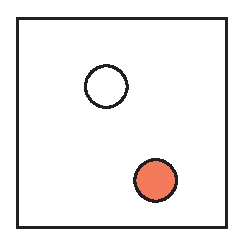
\includegraphics[width=1.5in]{sample.eps}
%  \caption{Lookit! Lookit!}
%}

%% Abstract section.
\abstract{ 
%
Augmented reality offers a means of overlaying interactive virtual
elements onto real world environments.  Further motivated by
%an interest in
%developing new methods for 
natural multi-user interactions in the context of games, we present
\emph{ARmy,} a proof of concept, two-player military strategy game 
%\fbox{proof of concept}
that 
%demonstrates the
%concept of 
combines physical tabletop games with virtual elements characteristic
of modern video games.
As players move plastic miniatures within a
physical environment, the application moderates and augments play by
maintaining a 3D representation of the scene, which it uses to
validate movement paths and perform automatic line-of-sight
calculations.
%
The ARmy application leverages a {\em table-top Spatially Augmented
  Reality} system 
%is built on top of a display system capable of
%dynamically augmenting the appearance of physical objects.  The system
%uses 
with a single overhead camera to track a collection of movable, white
surfaces, and applies virtual textures to these objects using six standard office 
%$multiple
projectors.  We describe some of the implementation details,
advantages, and limitations of the application. In addition, we
studied users interacting with the system to gauge the effectiveness,
intuitiveness, and robustness of the application. We describe the
process of this user study, and discuss results.
%We performed 
%\fbox{add a bit more about the user study}
%
} % end of abstract



%% ACM Computing Classification System (CCS).  
%% See <http://www.acm.org/class/1998/> for details.
%% The ``\CCScat'' command takes four arguments.

\CCScatlist{ 
  \CCScat{I.3.7}{Computer Graphics}{Three-Dimensional Graphics and Realism}{Virtual Reality}
}


%%% The ``\keywordlist'' command prints out the keywords.

%% Copyright space is enabled by default as required by guidelines.
%% It is disabled by the 'review' option or via the following command:
% \nocopyrightspace

%%%%%%%%%%%%%%%%%%%%%%%%%%%%%%%%%%%%%%%%%%%%%%%%%%%%%%%%%%%%%%%%
%%%%%%%%%%%%%%%%%%%%%% START OF THE PAPER %%%%%%%%%%%%%%%%%%%%%%
%%%%%%%%%%%%%%%%%%%%%%%%%%%%%%%%%%%%%%%%%%%%%%%%%%%%%%%%%%%%%%%%%


\renewcommand{\topfraction}{0.9}
\renewcommand{\bottomfraction}{0.9}
\renewcommand{\textfraction}{0.1}
\renewcommand{\floatpagefraction}{0.75}


\begin{document}

%% The ``\maketitle'' command must be the first command after the
%% ``\begin{document}'' command.  It prepares and prints the title block.

%% the only exception to this rule is the \firstsection command
\firstsection{Introduction}

\maketitle

%% \section{Introduction} 

Games are found throughout every day life in a variety of forms, and
can be a source of entertainment, a means for education, and even a
medium for artistic expression or social commentary.  Tangible
``tabletop games'' include a variety of board, card, and dice games,
such as chess, \emph{Monopoly}~\cite{Monopoly}, \emph{The Settlers of
  Catan}~\cite{Catan}, 
%\emph{Puerto Rico}~\cite{PuertoRico},
\emph{Magic: The Gathering}~\cite{MTG}, 
%\emph{Dungeons \&  Dragons}~\cite{D&D}, 
\emph{Warhammer 40,000}~\cite{Warhammer40k}.  These
games use physical pieces to facilitate play.  In contrast, modern
video games provide an experience that is purely virtual, allowing the
user to interact with a virtual game world that responds in realtime
with appealing visuals. Video games have the advantage of being autonomous agents, allowing for the incorporation of complex simulations with automatic rules enforcement. In contrast, tabletop games hold players responsible for moderating the game, which can be difficult and tedious. However, the physically tangible interfaces of tabletop games are often preferable to electronic input devices, which can be challenging and alienating to novice users.

Recent strides in the field of Augmented Reality (AR) have opened up
new ways for users to view and interact with virtual elements embedded
in the real world.  Our work is motivated by the possibility of AR
games that combine elements of tabletop games and video games to
create an exciting, new experience.  We present \emph{ARmy}
(Figure~\ref{FIGURE:GameInProgress}), an AR miniature war game played
using plastic soldier figurines and physical terrain models in a style
similar to \emph{Warhammer 40,000}.  Multiple projectors are used to
directly augment the play surface, displaying useful information about
the game state to the players and adding visual detail to the terrain.
An overhead camera tracks the movements of the game pieces, and a
semi-autonomous game module maintains the state of the game. This
ensures that the rules are correctly followed and removes the need for
players to perform tedious bookkeeping tasks, such as measuring
distances or rolling dice to resolve outcomes.

\vspace{0.1in}
%\newpage
\noindent
Our contributions presented in this paper:\vspace{-0.1in}

\begin{itemize}

\item The design of a table-top Spatially Augmented
  Reality game.\vspace{-0.1in}
  
\item Robust and modular system implementation of this game.\vspace{-0.1in}

\item User study directly comparing the efficiency of non-augmented
  and augmented versions of the game.\vspace{-0.1in}

\item Evaluation of the effectiveness of the \emph{ARmy} game in
  combining the advantages of tabletop games and video
  games.\vspace{-0.1in}


\end{itemize}

%We briefly survey some of the related work, both in relation to games
%and AR in general.  We describe the game play and interface of ARmy, and
%briefly discuss the underlying details of our multiprojector system.
%We detail the process of running user studies on the system, and
%discuss the results of the studies in relation to our goals.  Finally,
%we discuss current limitations of the system, as well as improvements
%to be made through future work.

% FIGURE SHOWING GENERIC PLAYING / POINTING
\begin{figure}[t]
\newcommand{\picwidth}{1.65in}
\resizebox{\picwidth}{!}{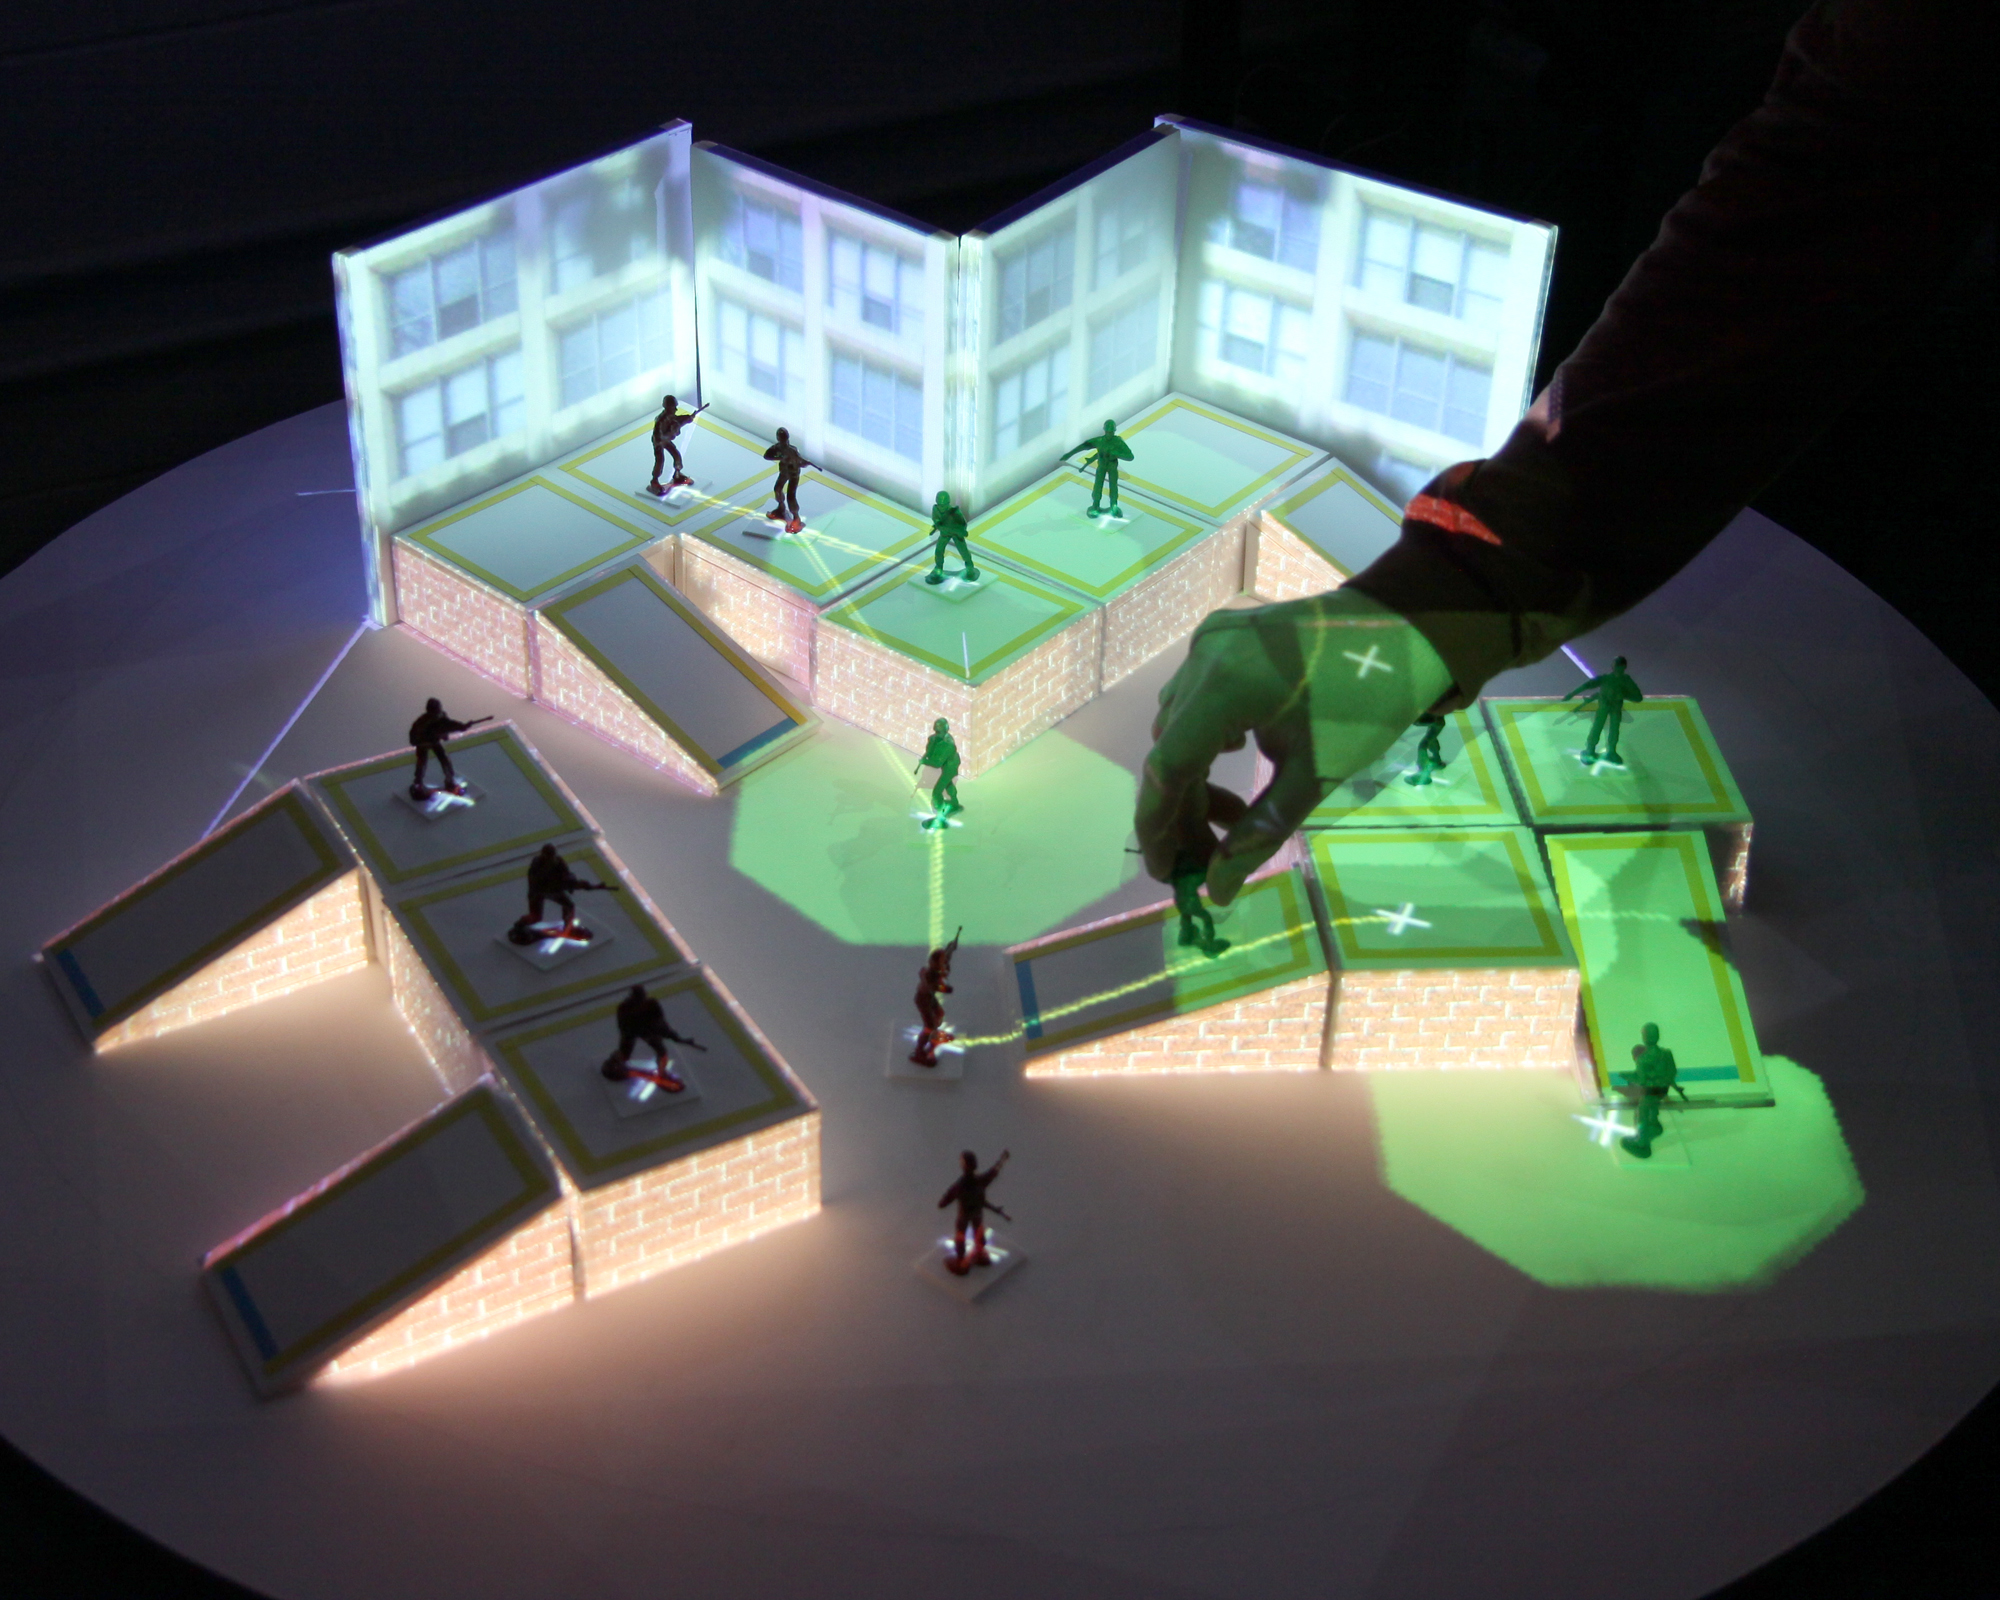
\includegraphics{images/greens_move_3.jpg}}\hspace{0.015in}%
\resizebox{\picwidth}{!}{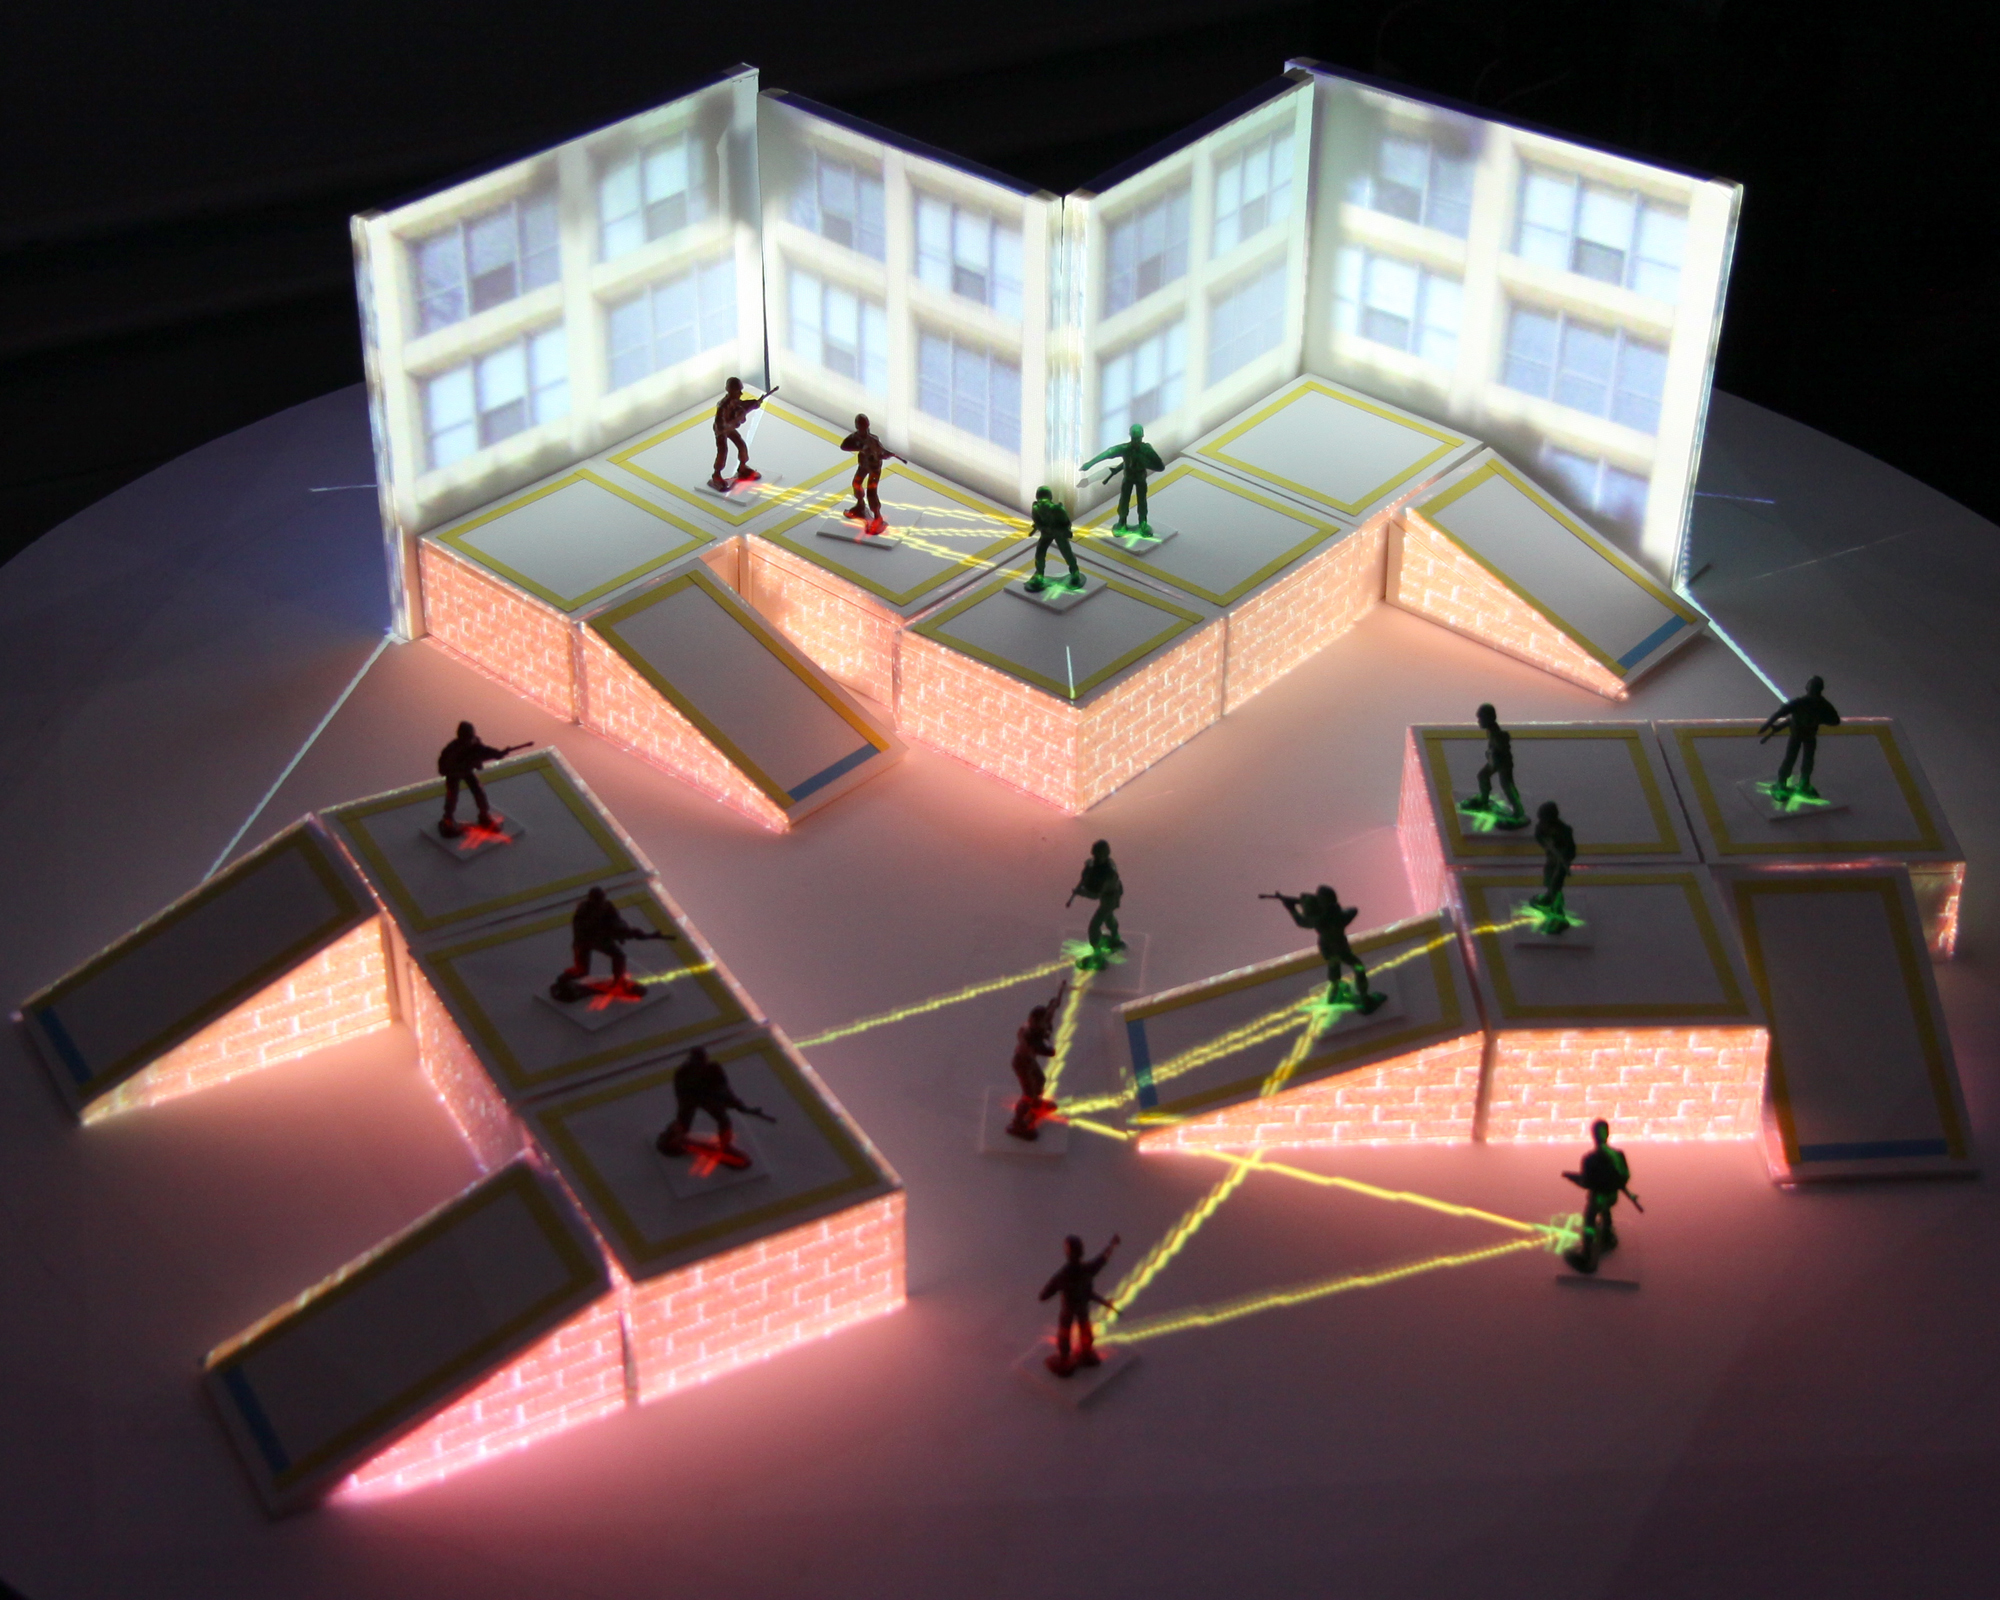
\includegraphics{images/lots_of_combat_2.jpg}}\\
\resizebox{\picwidth}{!}{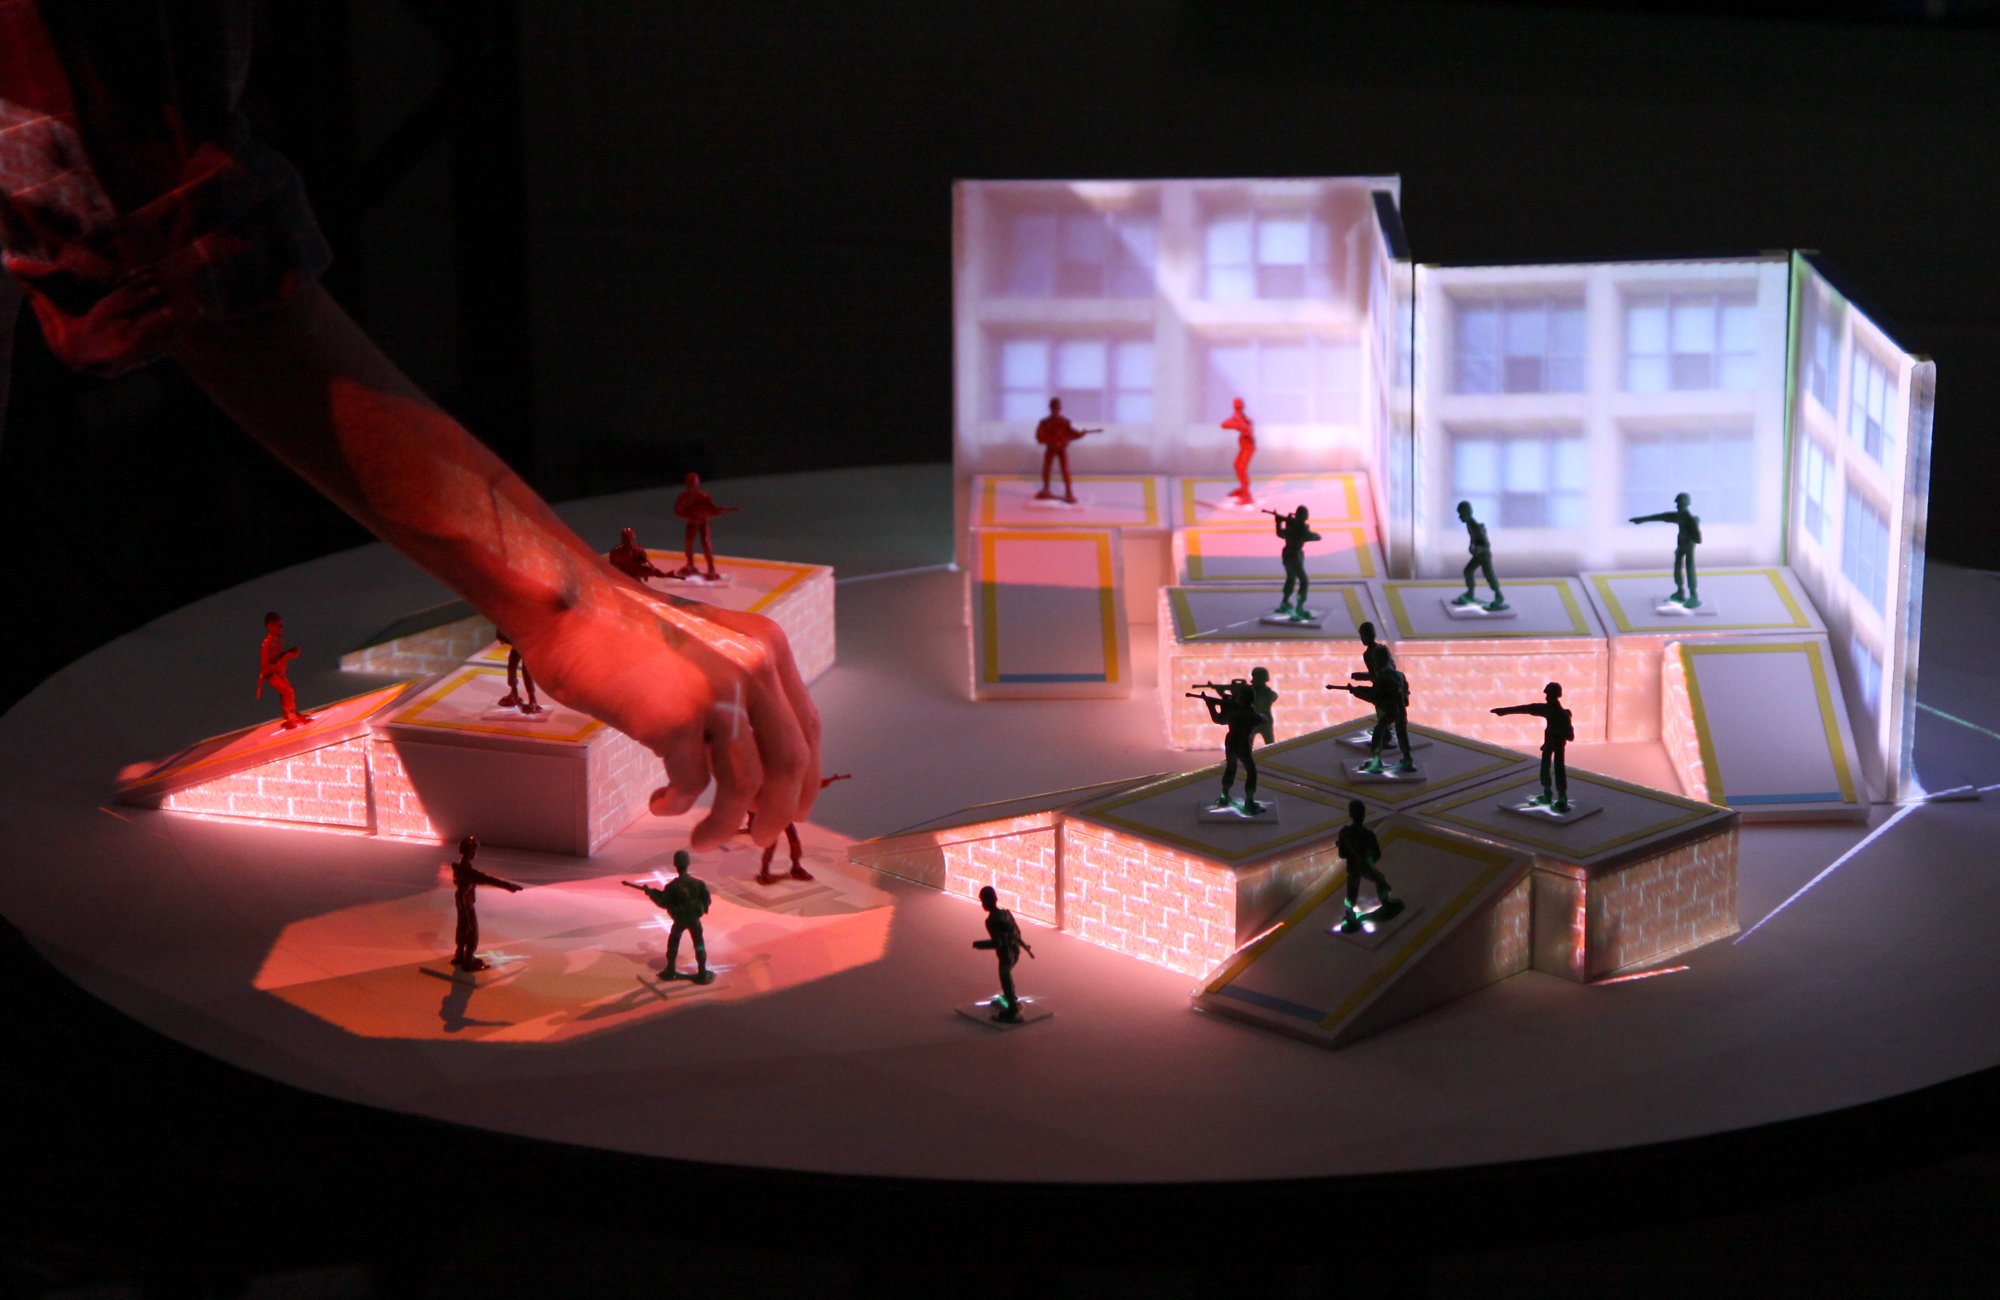
\includegraphics{images/reds_move.jpg}}\hspace{0.015in}%
\resizebox{\picwidth}{!}{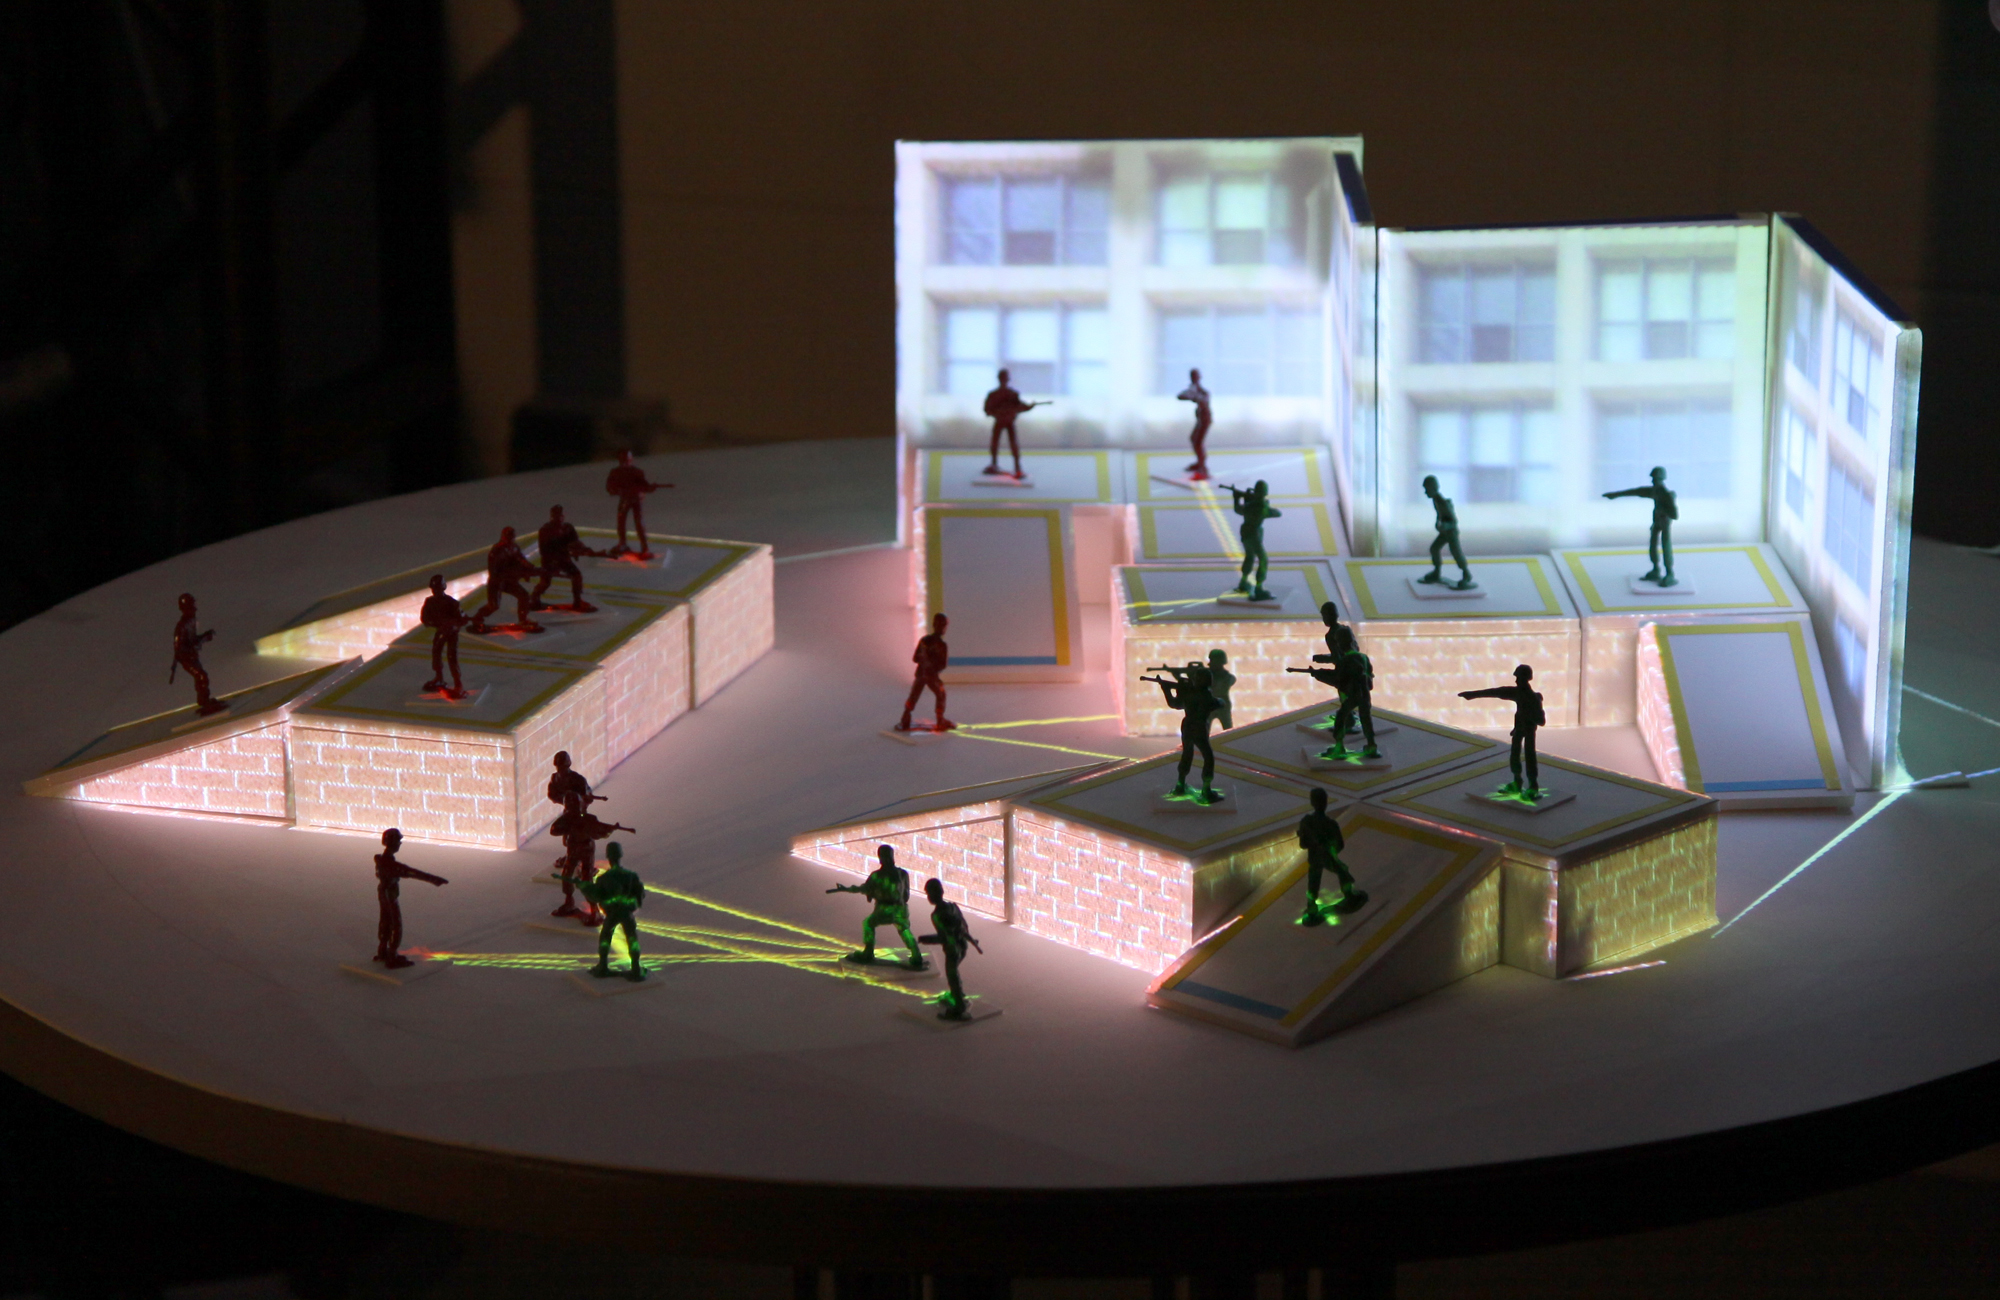
\includegraphics{images/lots_of_combat.jpg}}%
\vspace{-0.2in}\\
\caption[Images of ARmy: A Spatially Augmented Reality Game]{ The
  \emph{ARmy} game is an example of a spatially augmented reality game
  that combines physical game objects with virtual elements through
  projection.  The projections decorate simple, white objects with
  colorful virtual textures, and display important game information
  regarding legal moves and simulated combat.  }
\label{FIGURE:GameInProgress}
\vspace{-0.15in}
\end{figure}


\section{Related Work}

Augmented reality is a relatively recent field, with a large amount of
research focusing on how to combine the underlying technologies to
achieve stable, reproducible systems.  Two particularly important
problems that these systems must solve are the creation of an
effective augmented display, and the problem of 3D registration.

\subsection{Immersive Display Technology}

Existing AR systems use a variety of display techniques, which Bimber
and Raskar~\cite{BimberBook} classify into three main groups:
head-mounted, hand-held, and spatially aligned.  Head-mounted displays
are devices physically worn by the user, e.g.,
%Sutherlands's~
an optical see-though display~\cite{Sutherland1968} .  Hand-held
displays aim to use ubiquitous technology, such as Personal Digital
Assistants (PDAs)~\cite{Pasman2003, Wagner2003} and cell phones for
video see-through techniques.  Recent work has produced examples of
hand-held AR video games, such as \emph{ARhrrrr!}~\cite{ARhrrrr!},
%a game
%developed by the Georgia Tech Augmented Environments Lab and the
%Savannah College of Art and Design  The game is
played on a mobile device that overlays graphics onto a physical paper
map and incorporates tangible objects, such as brightly colored
candies.  A fully commercialized example of hand-held AR is the
Nintendo 3DS~\cite{Nintendo3DS}, which offers mobile AR games on an
autostereoscopic screen.

%\paragraph{Spatially Aligned Displays}

Our work is an example of \emph{Spatially Augmented Reality} (SAR), a
term coined by Bimber and Raskar~\cite{BimberBook} to describe AR
systems where the display devices are physically aligned and embedded
in the environment, instead of being attached to the user.  Some
spatial displays apply optical or video-based see-through techniques
by using stationary screens or monitors. For example,
% Bimber et
%al. present a 
the ``Virtual Showcase'' uses half-silvered mirror combiners to create
an enclosed AR display analogous to the physical showcases typical of
museum exhibits~\cite{Bimber2005}.

More closely related to our research are techniques which directly
augment the surfaces of physical objects using some configuration of
video projectors. An important and well-known example is the 
%CAVE
%``CAVE Automatic Virtual Environment'', 
%developed by
%Cruz-Neira et. al
CAVE~\cite{Cruz-Neira1993}.  Although the CAVE is technically
classified as an example of virtual reality, it stands as a
significant precursor to SAR techniques.  The display area is an
enclosed room comprised of rear-projection screens and a top-down
projector for displaying images on the floor, thus allowing for an
effective immersive environment.  The user is equipped with
head-tracking devices and 3D goggles for stereoscopic image display.

%Raskar et. al present 
The ``Office of the Future''
%, which
explores the possibility of using SAR applications in the setting of
an everyday workspace to facilitate telepresence and computing
tasks~\cite{Raskar1998a,Raskar1998b}.  
%They used 
%Multiple projectors present images on irregular, nonplanar surfaces,
%and demonstrated a technique for generating images suitable for such
%displays~\cite{Raskar1998b}.
%Their 
Later work expands upon these techniques with the idea of ``Shader
Lamps'', which allow for augmentation of complex 3D objects to create
the appearance of desired material properties, such as color and
texture~\cite{Raskar2000}.

A significant theme for much projection-based SAR research is the
vision of a future in which these display technologies have become
truly ubiquitous.  
%Underkoffler et al.  presented the idea of a
The ``Luminous Room'' is lit by multiple ``IO bulbs'', which combine a
projector and camera to facilitate both spatial display and user
interactions~\cite{Underkoffler1999}.  
%Pinhanez proposed the use of
``Everywhere Display'' projectors equipped with poseable mirrors allow
for the projection to be steered to any suitable surface within the
surrounding environment~\cite{Pinhanez2001}.  The idea behind each of
these techniques is to create a compact SAR device that can be
reasonably reproduced and distributed for use in homes, workplaces,
schools, commercial venues, and other public settings.



\subsection{3D Registration and Tracking}

In order to provide convincing visuals and a means for interaction,
the virtual objects and display devices must be registered in 3D
relative to the physical environment.  Generally this involves two
main steps: calibration and tracking.

%\subsubsection{Calibration}

Calibration refers to the problem of correctly modeling and recovering
geometric correspondences between display or tracking devices and the
physical environment.
%% In the case of projector-based displays, it is necessary that we be %% able to map each projector pixel to a known point relative to the %% world coordinate system so that we can use that information to project %% images that are correctly aligned with the physical display surfaces.  %% In addition, since camera devices are required for vision-based %% techniques used in the tracking step, these devices must also be %% calibrated.
%Camera and projector calibration is a classic vision topic that has
%been researched thoroughly.  
Typically cameras and projectors are described using the pinhole
model, which maps 3D points in the world to 2D image coordinates using
both intrinsic parameters, which describe center, scale, and skewness
of the image coordinate system, and extrinsic parameters, which
describe the rotation and translation of the camera relative to world
coordinates.  Zhang~\cite{Zhang2000} provides
a simple, robust method
for calibration in which the user captures multiple images of a
single, planar calibration target from differing points of view.  
The
method requires no a priori knowledge of the position, orientation, or
movement of the target relative to the camera.  
%Additional research
%Scaramuzza et al.~\cite{Scaramuzza2006} focus on recovering
%Calibration parameters involving significant lens distortion,
%specifically omnidirectional cameras, as well as cameras equipped with
%a fisheye lens.

%\subsubsection{Tracking}

\begin{figure}[t]
\newcommand{\picheight}{1.65in}
%\resizebox{!}{\picheight}{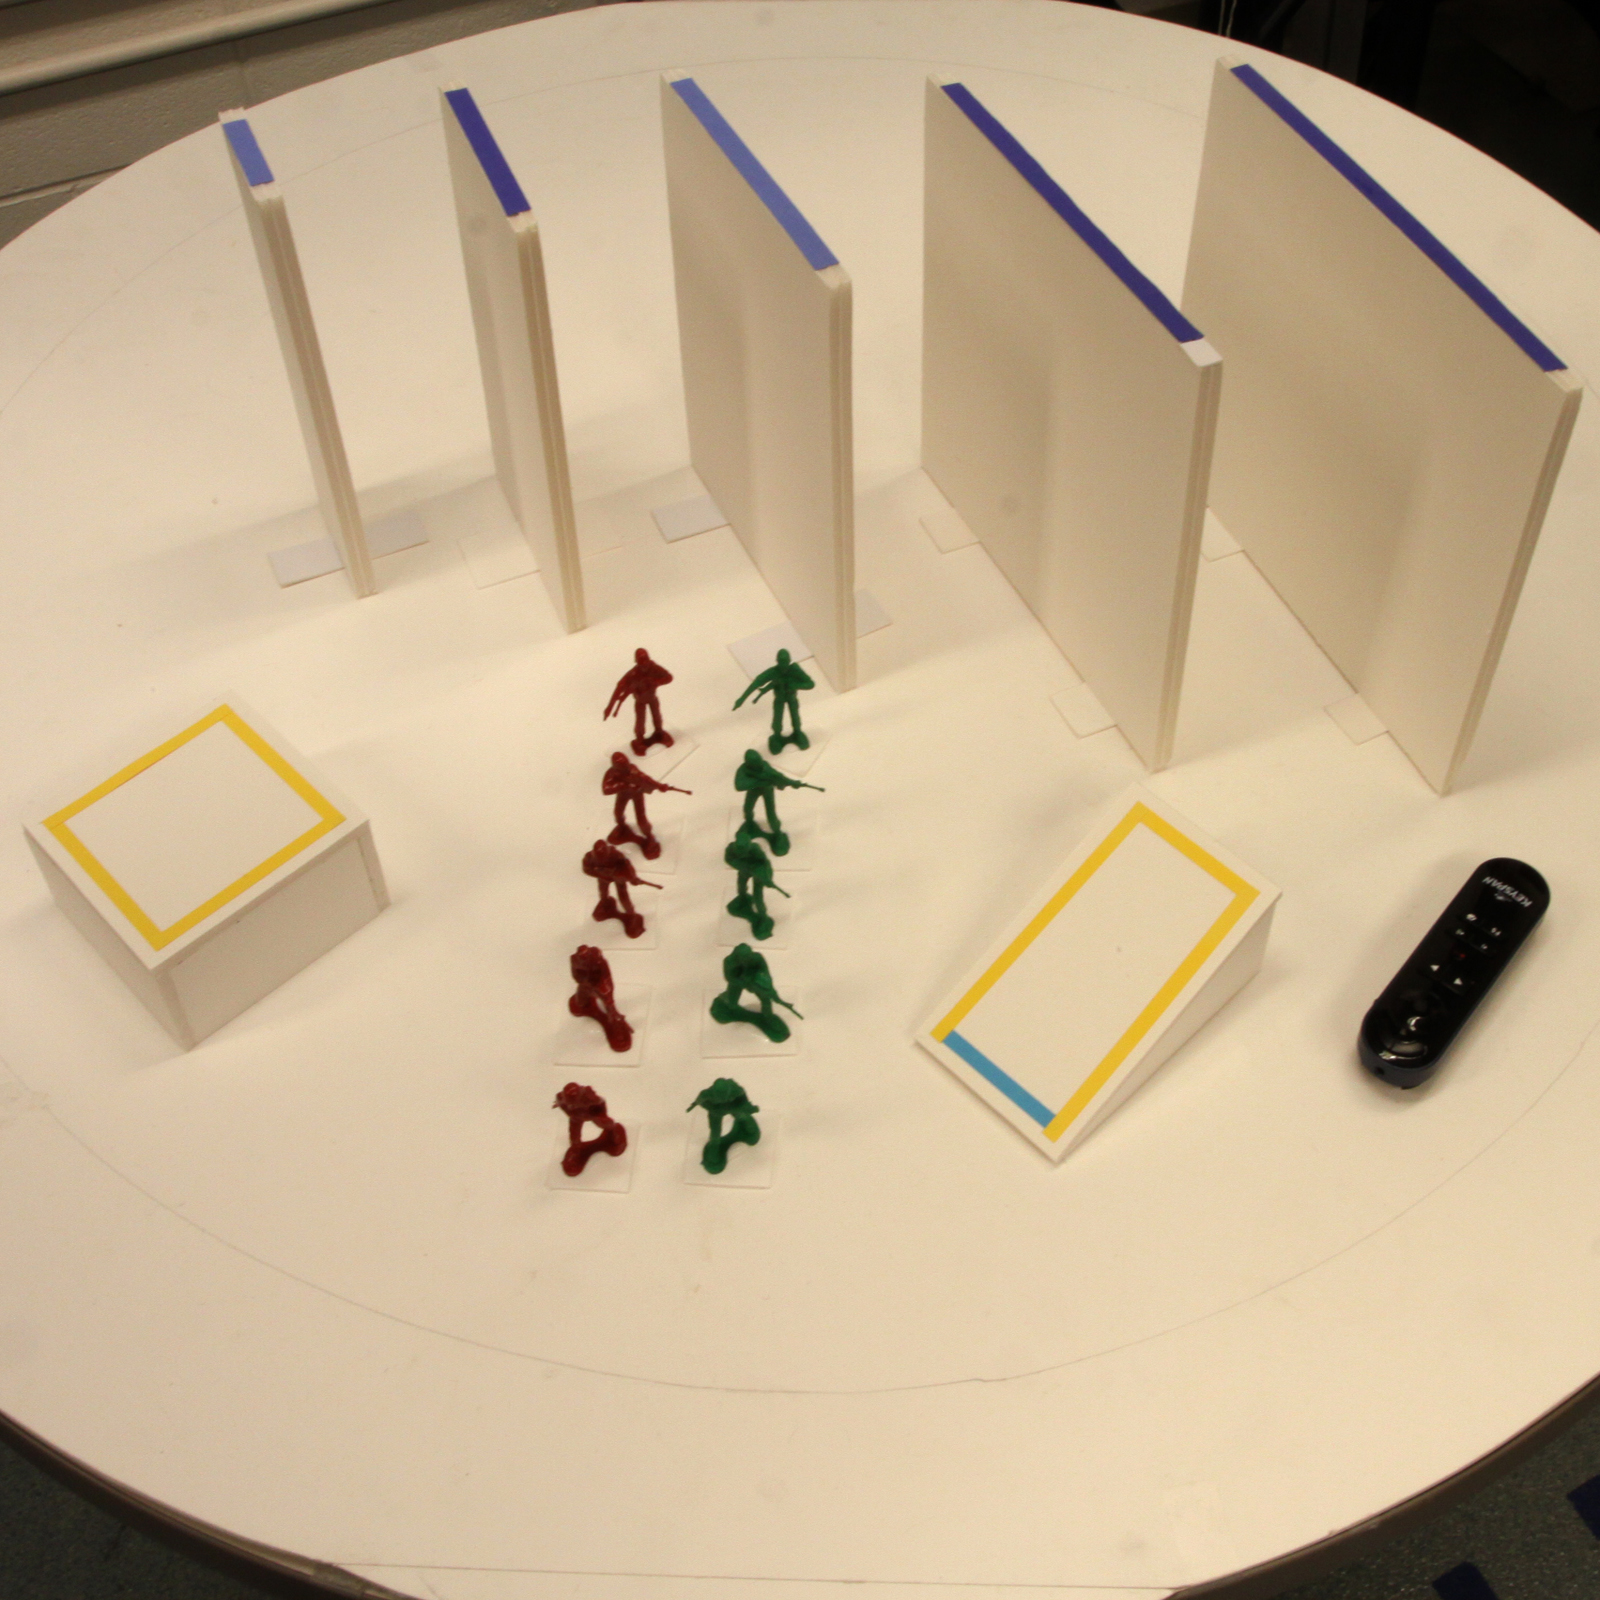
\includegraphics{images/props_crop.jpg}}
\resizebox{!}{\picheight}{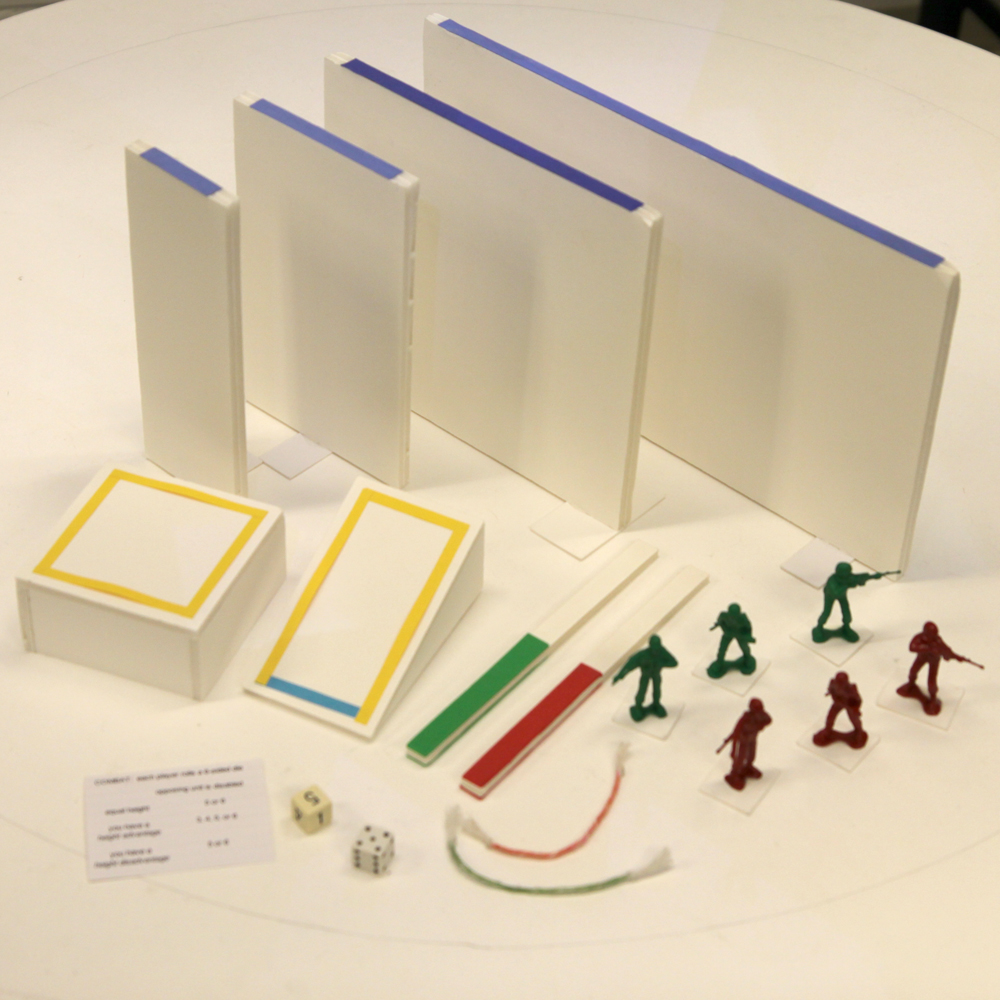
\includegraphics{images/props_2.jpg}}
\resizebox{!}{\picheight}{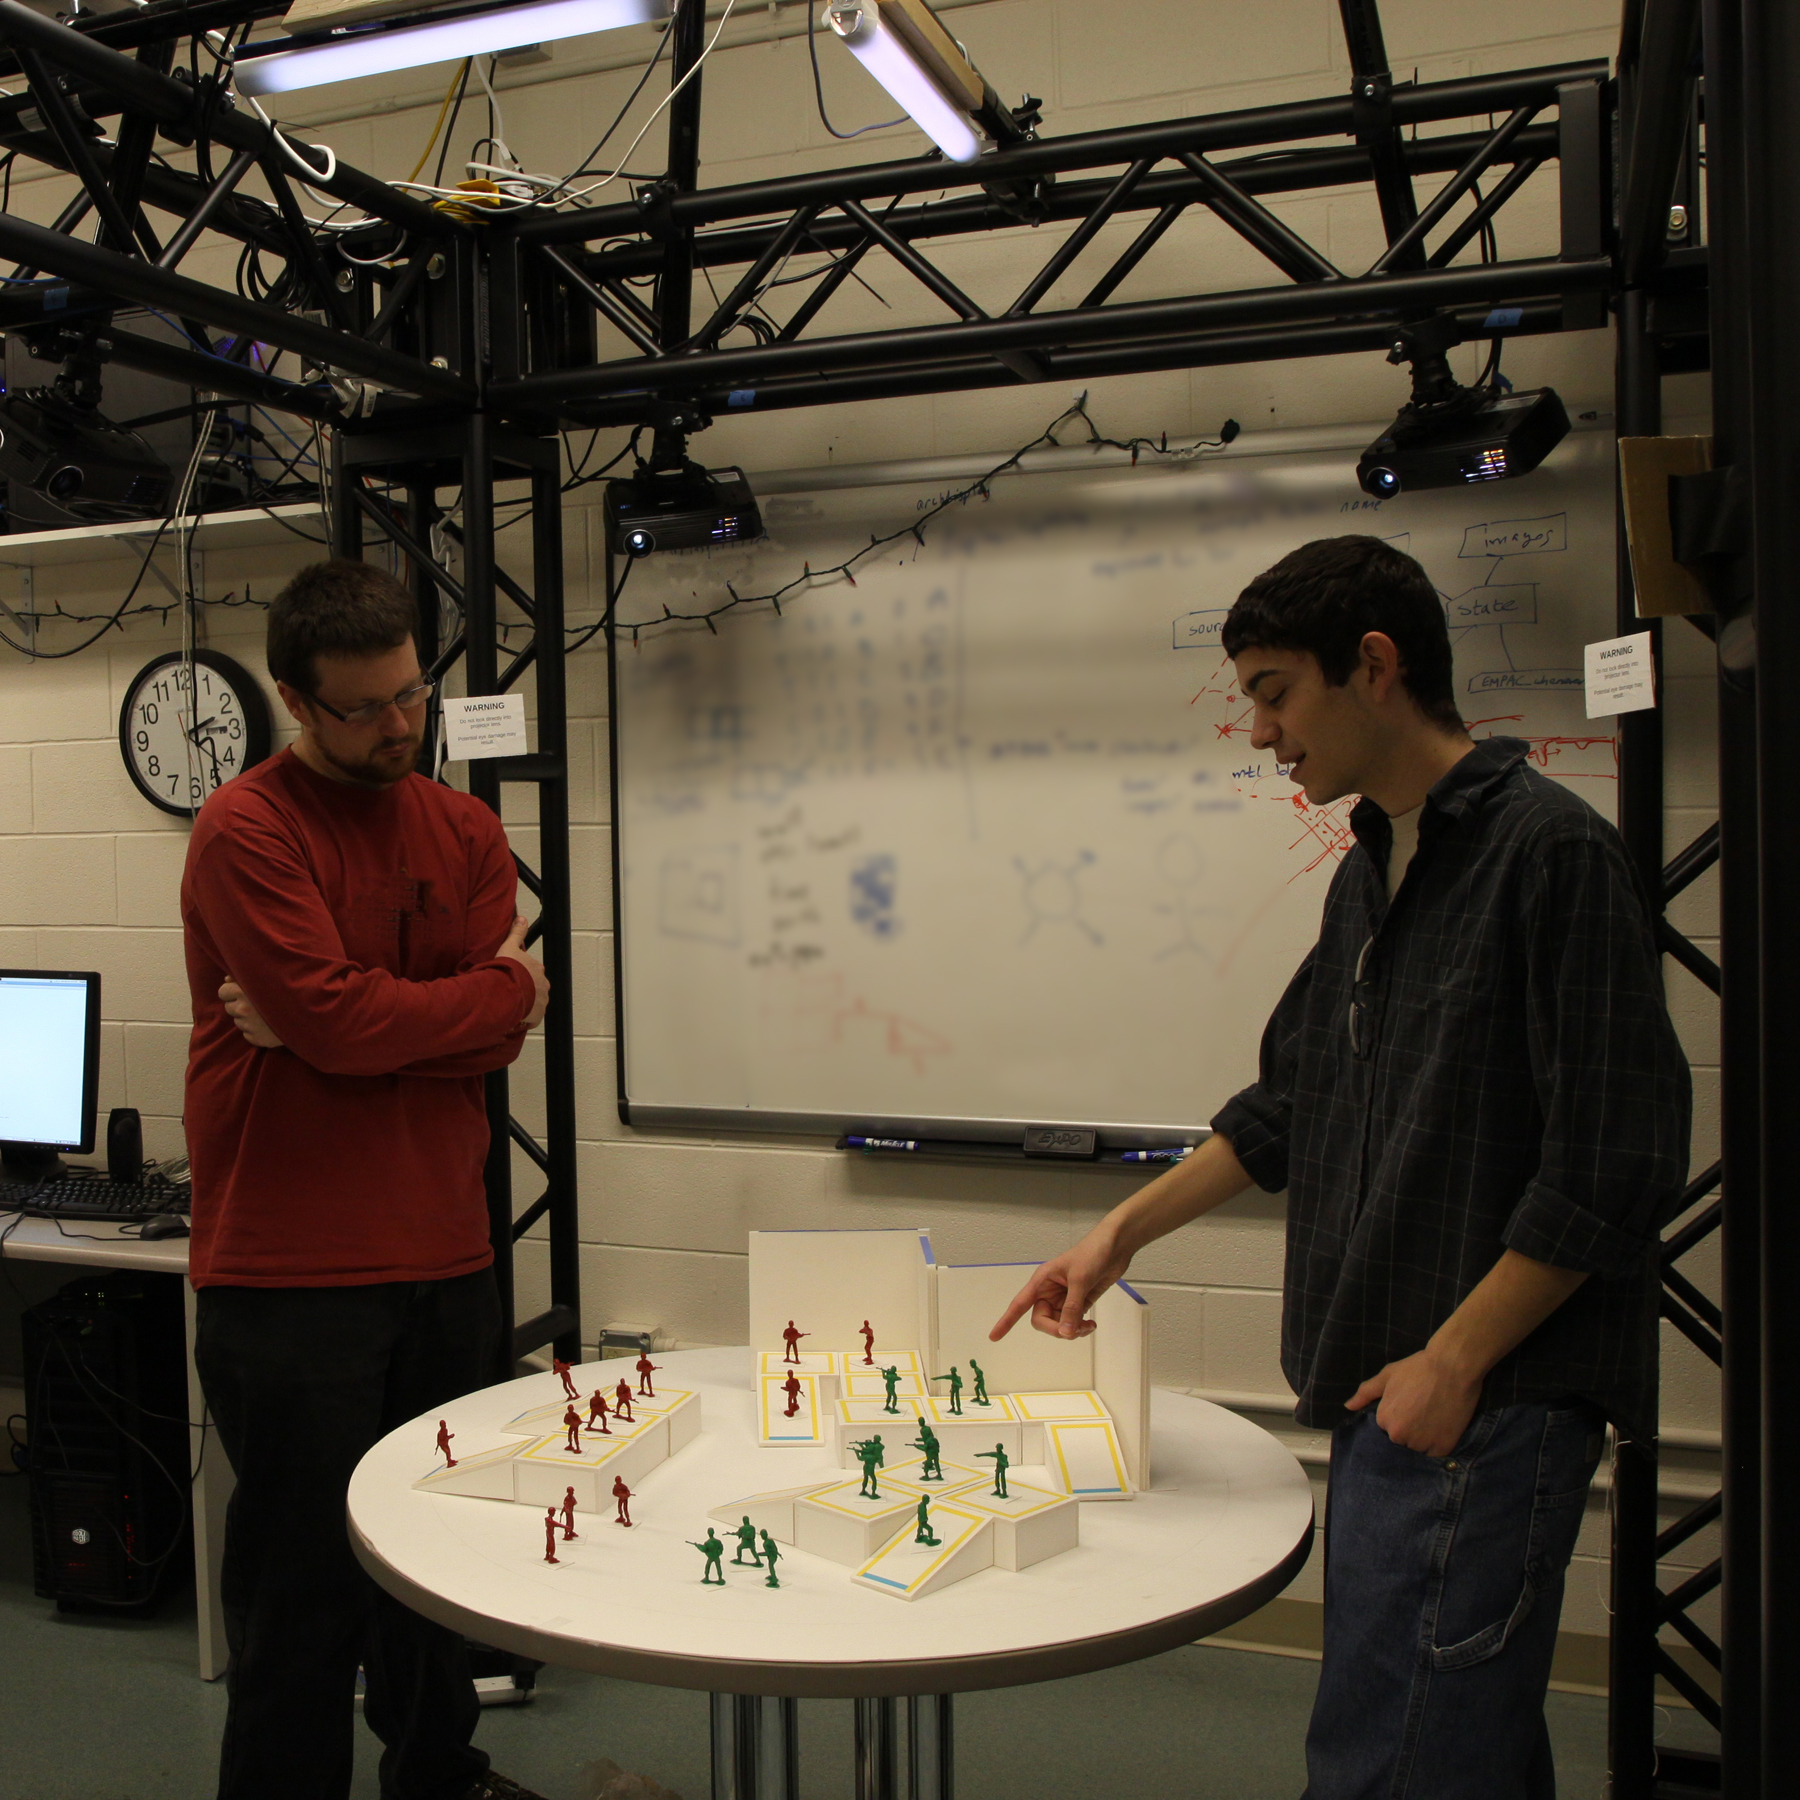
\includegraphics{images/contraption_with_people_blur.jpg}}%
\vspace{-0.1in}
\caption{ARmy is played using a set of physical 
%props 
%and a simple
%  wireless remote.  The prop library contains plastic soldier
  soldier figurines and foam-core terrain objects, including walls,
  platforms, and ramps.  The non-augmented version is played with measuring sticks \& string and dice.  
%\fbox{add string, sticks, and dice to left picture}
The spatially augmented reality version is equipped with a overhead
single camera for object detection and multiple projectors for
display.  
%It is designed to fully cover the surface of a centered
%table, which acts as a space for user interactions.  
}
\vspace{-0.1in}
\label{FIGURE:props_and_contraption}
\end{figure}

Once the display and vision devices are properly calibrated within the
world coordinate system, we can use them to accomplish tracking of
physical objects for augmentation.  Unlike calibration routines, which
typically are done once during setup, and therefore can accommodate
somewhat time-consuming, manual tasks, tracking must be done
automatically and efficiently at interactive rates for the system to
be responsive.  Registration and tracking can be accomplished using
electromagnetic and mechanical tracking devices~\cite{Cruz-Neira1993}
or using a variety of vision-based techniques, which are discussed
below.

%% \paragraph{Fiducial Markers}

A large variety of AR applications use fiducial markers to identify
objects and determine their position and orientation.  Kato and
Billinghurst~\cite{Kato1999} provide a method for tracking square,
planar markers with a black border and bi-tonal interior pattern.
%Their method identifies markers in the camera image by using
%edge-based vision techniques to detect quadrilaterals.  Detected
%regions are normalized, sampled, and compared via correlation to a set
%of marker patterns provided a priori by the user.  
%They present their
%technique in the context of an augmented reality conferencing system,
This software was released as ARToolkit, and has since become
well-known and widely used within the AR community.  ARTag, a similar
quadrilateral-based method developed by Fiala~\cite{Fiala2005}, uses
an extensive library of predefined marker codes to achieve increased
robustness in cases of partial occlusion. 
%\fbox{ Added stuff
%  here... should I have?}
%employs digital processing techniques to identify square markers
%bearing ten-digit identification codes, encoded in the form of
%six-by-six bitonal grids similar to barcodes.  This tracking system,
%known as ARTag, provides the user with a large library of predefined
%markers, and leverages redundancies in the encoding technique to
%identify markers even under conditions of partial occlusion.
%
Fiducial marker systems hold great promise for AR game applications,
as they provide a viable, inexpensive means of identifying specific
game-related objects.  For example, markers could be printed on cards,
attached to wooden game pieces, or positioned at the corners of a
movable game board.
% in a manner similar to the augmented whiteboard
%used in Kato and Billinghurst's conferencing system~\cite{Kato1999}.
One disadvantage of fiducial markers is that the robustness and
accuracy of the tracking generally depends on the relative size of the
markers in the camera image.
%, since an image of a marker that is too
%small or far away may not yield sufficient resolution for the tracking
%algorithm to identify the contained pattern.  
Thus, suitable tracking may require markers that are too large or
unwieldy for players to use comfortably.  In addition, large fiducial
markers may interfere with the visual quality of virtual elements
projected onto them.  This presents an added problem for
projector-based SAR systems, which, unlike see-through AR displays,
cannot fully hide the marker with rendered objects.


\begin{figure*}[t]
\begin{center}
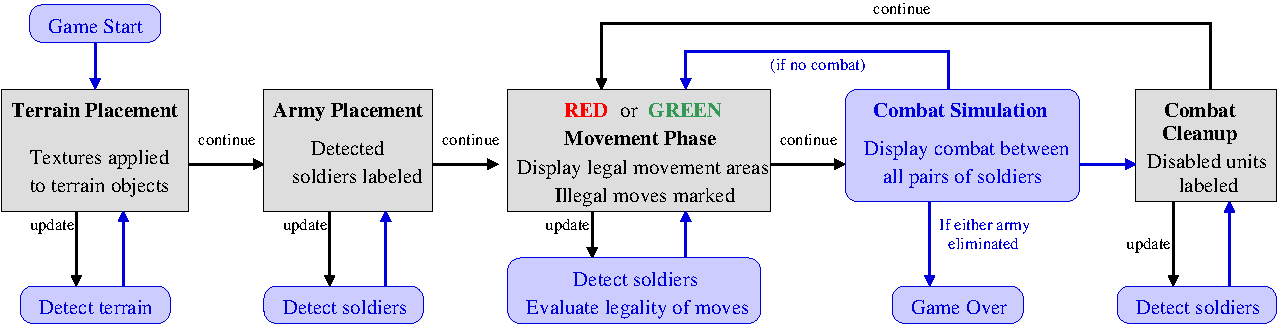
\includegraphics[width=7.0in]{images/game_diagram_horizontal.pdf}
\end{center}
\vspace*{-0.15in}
\caption[ARmy Application State Diagram]{State diagram of the
    ARmy application.  Gray boxes represent stages of play defined by
    player actions.  Blue boxes represent stages performed completely
    by the game module.  Similarly, black arrows represent transitions
    triggered by the players via the remote control, while blue arrows
    represent automatic transitions.}
\label{FIGURE:ARmyDiagram}
\vspace{-0.1in}
\end{figure*}



Other useful methods for 3D registration employ structured light
techniques, which project known pixel patterns into the scene and
measure the result in order to recover depth information.  Ashdown et
al.~\cite{Ashdown2004} use a variation of structured light to project
successive patterns containing continuous horizontal and vertical
lines.  
%The method detects ``kinks'' in the lines and uses this
%information to segment the image into multiple planar regions, which
%are then stitched together into a continuous display by refining their
%individual homographies to fit adjacency constraints.  
Lee et al.~\cite{Lee2004} propose a structured light method for
registering projection surfaces 
%without the use of a camera and vision
%techniques.  Instead, 
by embedding light sensors in the corners of the target surface
% are embedded
The sensors detect patterns projected onto the surface and
%with light sensors, which detect and transmit the binary sequences
%projected in the patterns.  The system 
use this information to track the 3D position of the object.
%identify the quadrilateral region of the
%surface within the projector image and warps images accordingly.

%% \paragraph{Imperceptible Pattern Embedding}

%% A potentially serious hurdle for the application of fiducial marker %% and structured light techniques to display systems that use direct %% augmentation is interference from projected images.  In other words, %% projecting a colored image onto a surface bearing a fiducial marker %% may obscure the pattern of the marker in such a way as to prevent %% correct identification by the tracking algorithm.  Projected structured %% light patterns suffer from the same problem, and may obstruct the %% displayed images or otherwise distract the user.  

%% One possible solution to this problem involves directly embedding %% structured light patterns into the display images in such a way as to %% remain imperceptible to the user.  Lee et al.~\cite{Lee2005} %% demonstrate an improvement on their previous sensor-based technique %% which is able to embed the light patterns into perceptually uniform %% gray blocks, which are less distracting than high-contrast patterns.  %% Although the method is shown to achieve accurate tracking at %% interactive framerates, regions bearing the embedded patterns are %% still visible to the user and reduce the overall display space %% available for application content.  In addition, the method is shown to %% work only with a modified projector that outputs grayscale images.

%% Cotting et al.~\cite{Cotting2004} propose a method that achieves %% direct pattern embedding by taking advantage of unmodified DLP %% projectors, which use precisely-timed modulation of micro-mirrors to %% determine the intensity and color of each image pixel.  Each pixel %% corresponds to a single mirror, which switches between a ``white'' %% position that tilts toward the projector light source, thus %% contributing high intensity light to the image, and a ``black'' %% position that tilts away, thus contributing little light.  Their method %% first measures the sequences of mirror flips across the full range of %% color values for each independent color channel.  Then it remaps each %% pixel to a perceptually similar color value such, that during a %% predetermined exposure time, the mirror's position matches the %% specified black or white value of the desired light pattern.  Using %% carefully calibrated exposures, the camera can acquire images of the %% light pattern without greatly degrading the image quality of the %% simultaneous display.  Although appealing, short-exposure methods such %% as this require the extra work of precisely synchronizing the camera %% and projectors.

%% \paragraph{Infrared Tracking}

With SAR systems, vision-based tracking techniques often encounter a problem when projected images interfere with object tracking. One solution is to track objects with infrared light,
%based only on specific wavelengths of
%light which are not projected in significant amounts by the display.
%A significant amount of research has experimented with tracking using
%infrared light,
which is invisible to the human eye and therefore does not interfere
with displayed images~\cite{Lee2007,Kinect}.

%have
%presented the use of a hybrid LED projector capable of transmitting
%both infrared and visible light in order to simultaneously display
%visible application images and invisible structured light patterns.
%Although an excellent proof of concept, the proposed method does not
%work with standard commodity projectors.
%
%More recent work has led to the development of commercially available
%3D range cameras, which use infrared structured light techniques to
%produce real-time depth images of a measured scene.  Perhaps the most
%widely known example of this kind of registration is Microsoft's
%Kinect, a recent Xbox 360 peripheral that uses a depth-image camera as
%an input device for motion-based controls~\cite{Kinect, Shotton2011}.
%A different approach to infrared-based tracking is to use more
%conventional infrared-emitting devices, such as LED markers or laser
%pens.  Kato and Billinghurst demonstrated the use of an infrared
%LED-tipped stylus that allowed users to interact with a virtual
%whiteboard~\cite{Kato1999}.  The LED activates in response to pressure
%on the tip of the stylus, and is detected by a calibrated infrared
%camera.  Because the surface location of the whiteboard is known, the
%system is able to determine the location of the pen tip in screen
%coordinates, allowing the user to write or draw on the augmented
%display.
%
%\paragraph{Color-based Tracking}
%
Finally, color information provides another potential means for detecting and
registering objects.  For example, the Luminous Room project presented
by Underkoffler et al.~\cite{Underkoffler1999} used a simple tagging
system through which application-specific objects were marked with
small groupings of colored dots.  The system identifies objects by
first detecting dots as regions of specified size and color, and then
by grouping individual dots based on patterns with known distance and
angle constraints.

%% An advantage of color-based techniques is that they are generally %% simpler to implement and at times faster than more sophisticated %% vision algorithms.  




One problem of color-based techniques is that they may not be highly
robust under inconsistent lighting conditions, and are likely to
suffer from a high number of false positives, as target colors may
appear within background clutter.  
%The Luminous Room prototype avoids
%these problems by using special reflective dot markers which appear
%brighter in the camera image, allowing them to be easily separated
%from the background.  In addition, colored markers share the same
%problem as bitonal fiducial markers, in that projected visuals are
%likely to obscure the appearance of the marker, making it difficult to
%achieve simultaneous capture and display.  
Despite these drawbacks, color-based object recognition may be useful
in the context of SAR games, since color is commonly used in board and
card games to distinguish objects that appear otherwise identical.
Thus it might be possible to track existing game pieces without the
need for additional annotation.

% \paragraph{Human Tracking}

%% In addition to tracking physical game pieces, another set of %% interactions can be achieved through the tracking of the users.  
%% For example, the Kinect tracks the user's body and maps it to a %% skeleton model in real time, allowing for game applications to use %% full-body gestural controls~\cite{Shotton2011, Kinect}.  Other research %% has tried to achieve accurate tracking of specific body parts, most %% commonly focusing on the human hand.  Lee and H\"{o}llerer present %% Handy AR, a system for markerless tracking that detects and estimates %% the 3D pose of an out-stretched human hand~\cite{LeeT2007}.  This %% provides the benefit of allowing the user's hand to act in place of a %% fiducial marker, but requires the hand to remain out-stretched during %% use.  More recently, Wang and Popovi\'c~\cite{Wang2009} have proposed %% using a lightweight colored glove to allow for more robust detection %% of a wide variety of hand poses, including such complex gestures as %% the alphabet used in American Sign Language.




\section{ARmy Simulation Overview}

The ARmy application is a military simulation game played between two
opponents.  The players are given a number of plastic soldier
figurines, referred to as \emph{units}, which represent their
respective armies (Figure~\ref{FIGURE:props_and_contraption}).  Each
player moves his units through the scene according to the rules of the
game, engaging in combat with opposing units to eliminate them from
play.  Victory is achieved by completely eliminating the opposing
army, or by having the most units at the end of a set time limit.



Most tabletop games are played over a number of turns consisting of
multiple steps, through which the players progress at their own pace.
In the same way, the ARmy application is designed as a series of
player-controlled feedback loops, meaning that the game module only
proceeds at the request of the players.  The current implementation
relies on a simple wireless remote control, which allows the players
to send two different signals to the game module.  The first is an
{\em update request} that tells the game to capture a new image, 
detect the current physical game state, and
visualize any new information.
%update its model of the scene and
%display any new information.  
The second is a {\em continue} command, which indicates that the
players have finished with the current stage of play and wish to
proceed to the next step.  Figure~\ref{FIGURE:ARmyDiagram} diagrams
the overall design of the interaction using a finite state
representation.



%In designing this application, special consideration was given as to %how SAR techniques could be leveraged to improve upon the play style %of traditional tabletop games.  This section provides a step-by-step %description of how the game is played, as well as how it incorporates %virtual elements to create a new and interesting game experience.



\subsection{Terrain Placement}


%% %FIGURE : TERRAIN DETECTION IMAGES
\begin{figure}[b]
\newcommand{\picwidth}{1.65in}
 \resizebox{\picwidth}{!}{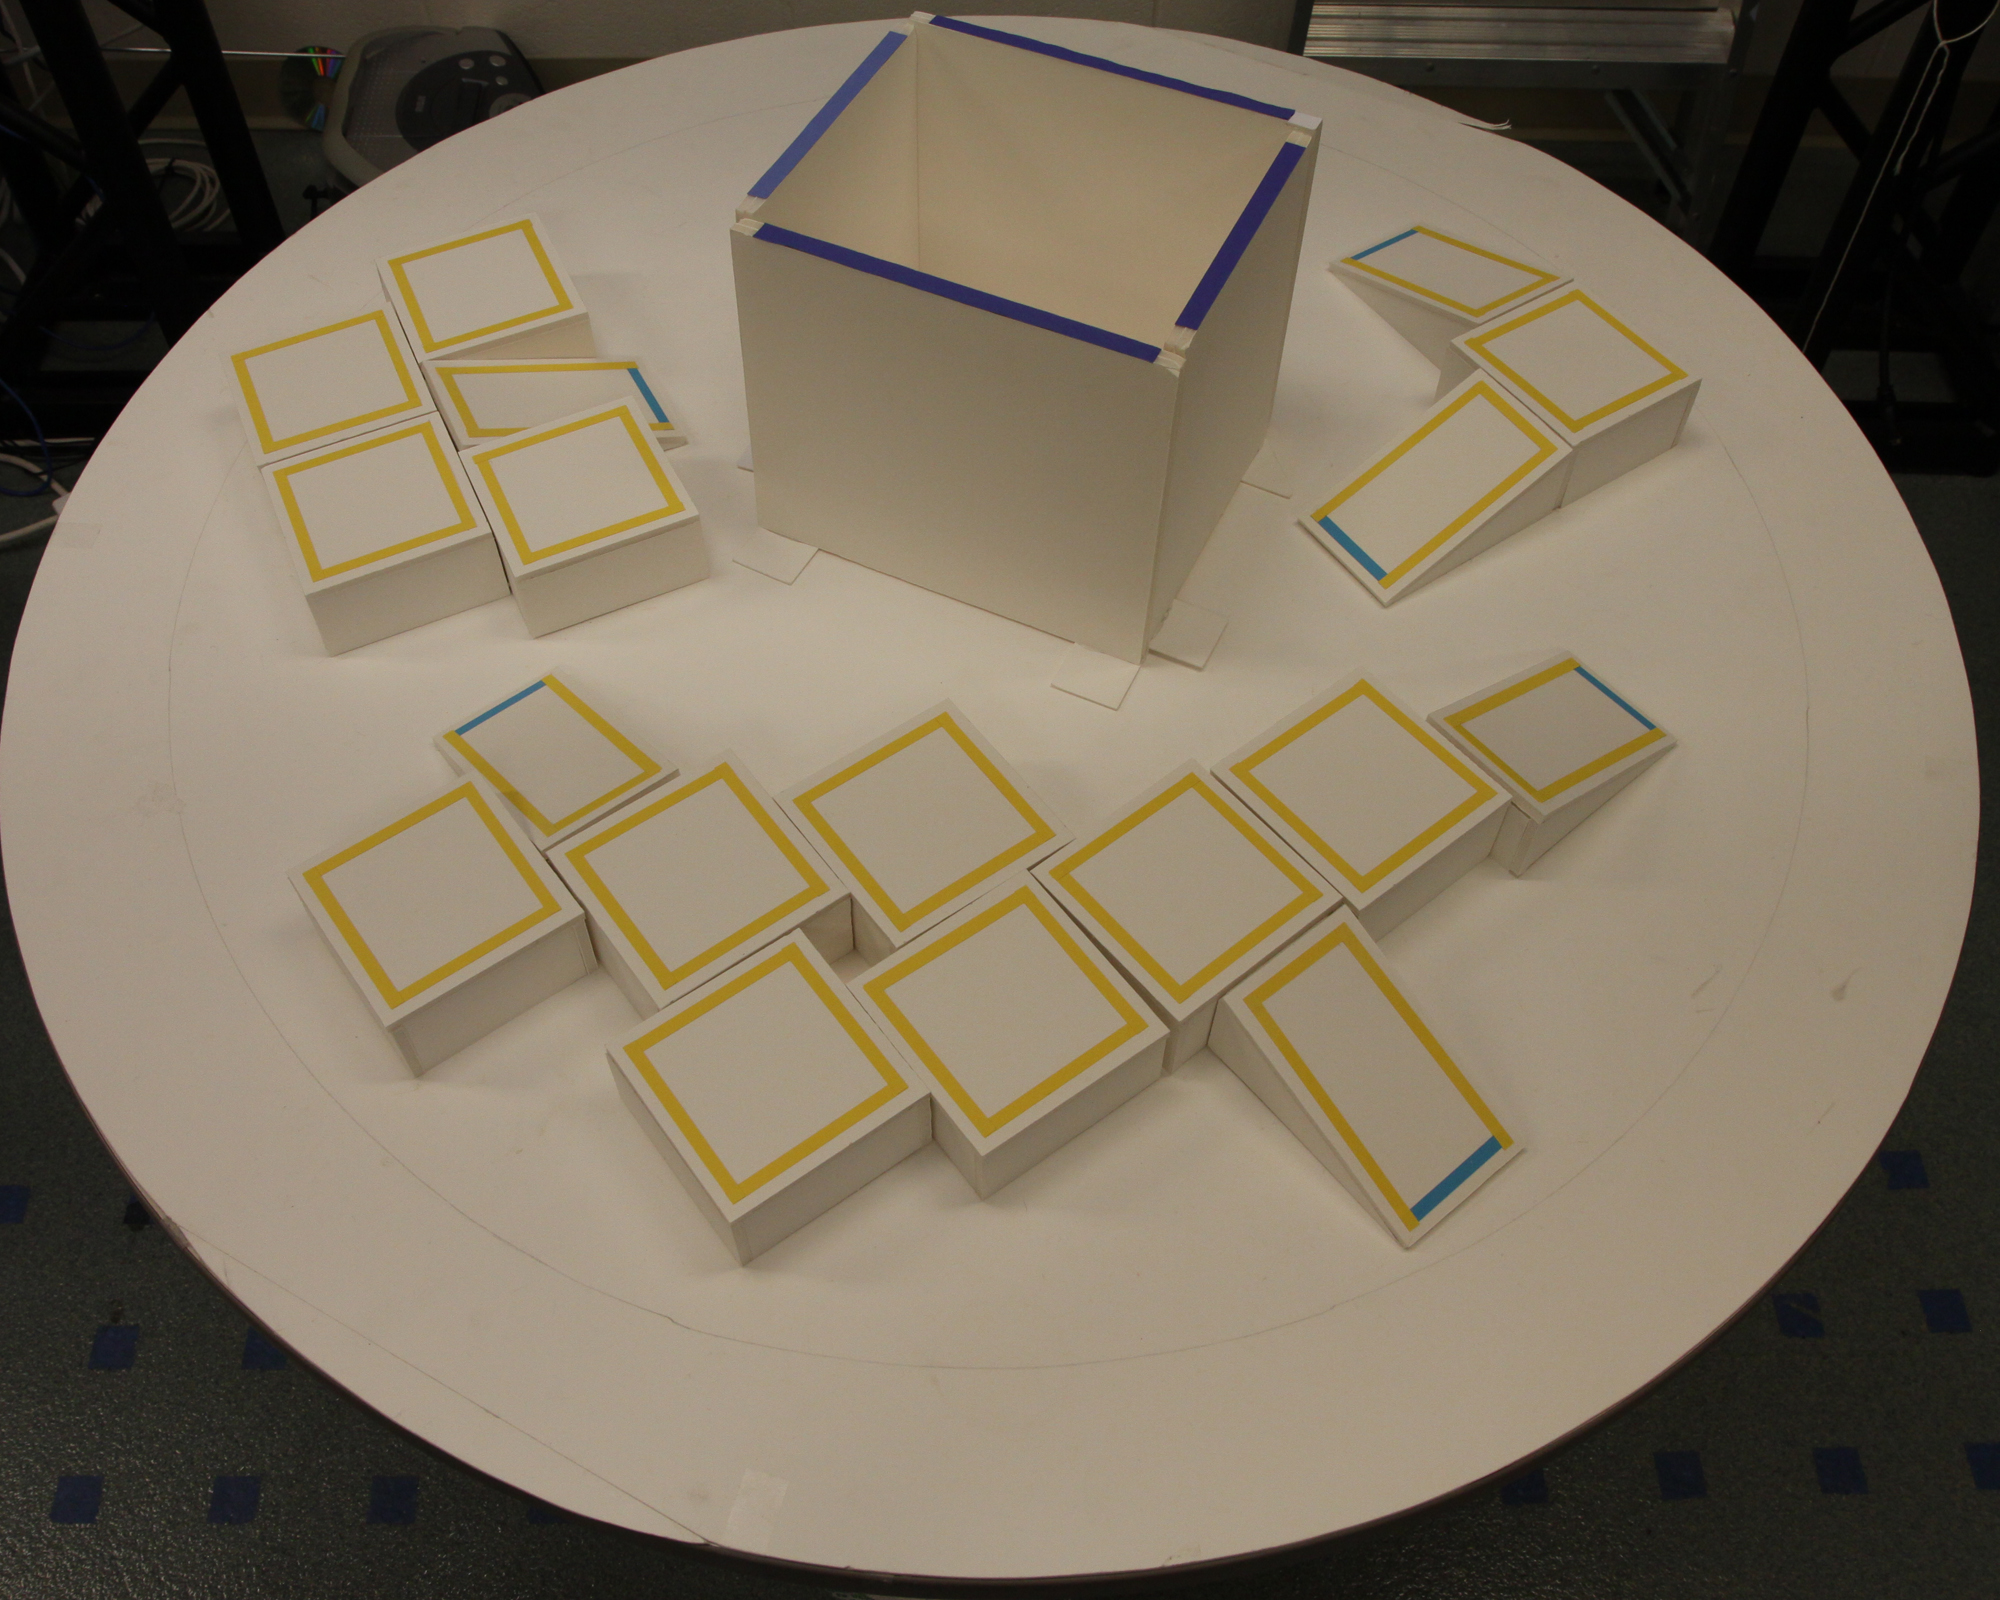
\includegraphics{images/complex_lights_on.jpg}}
 \resizebox{\picwidth}{!}{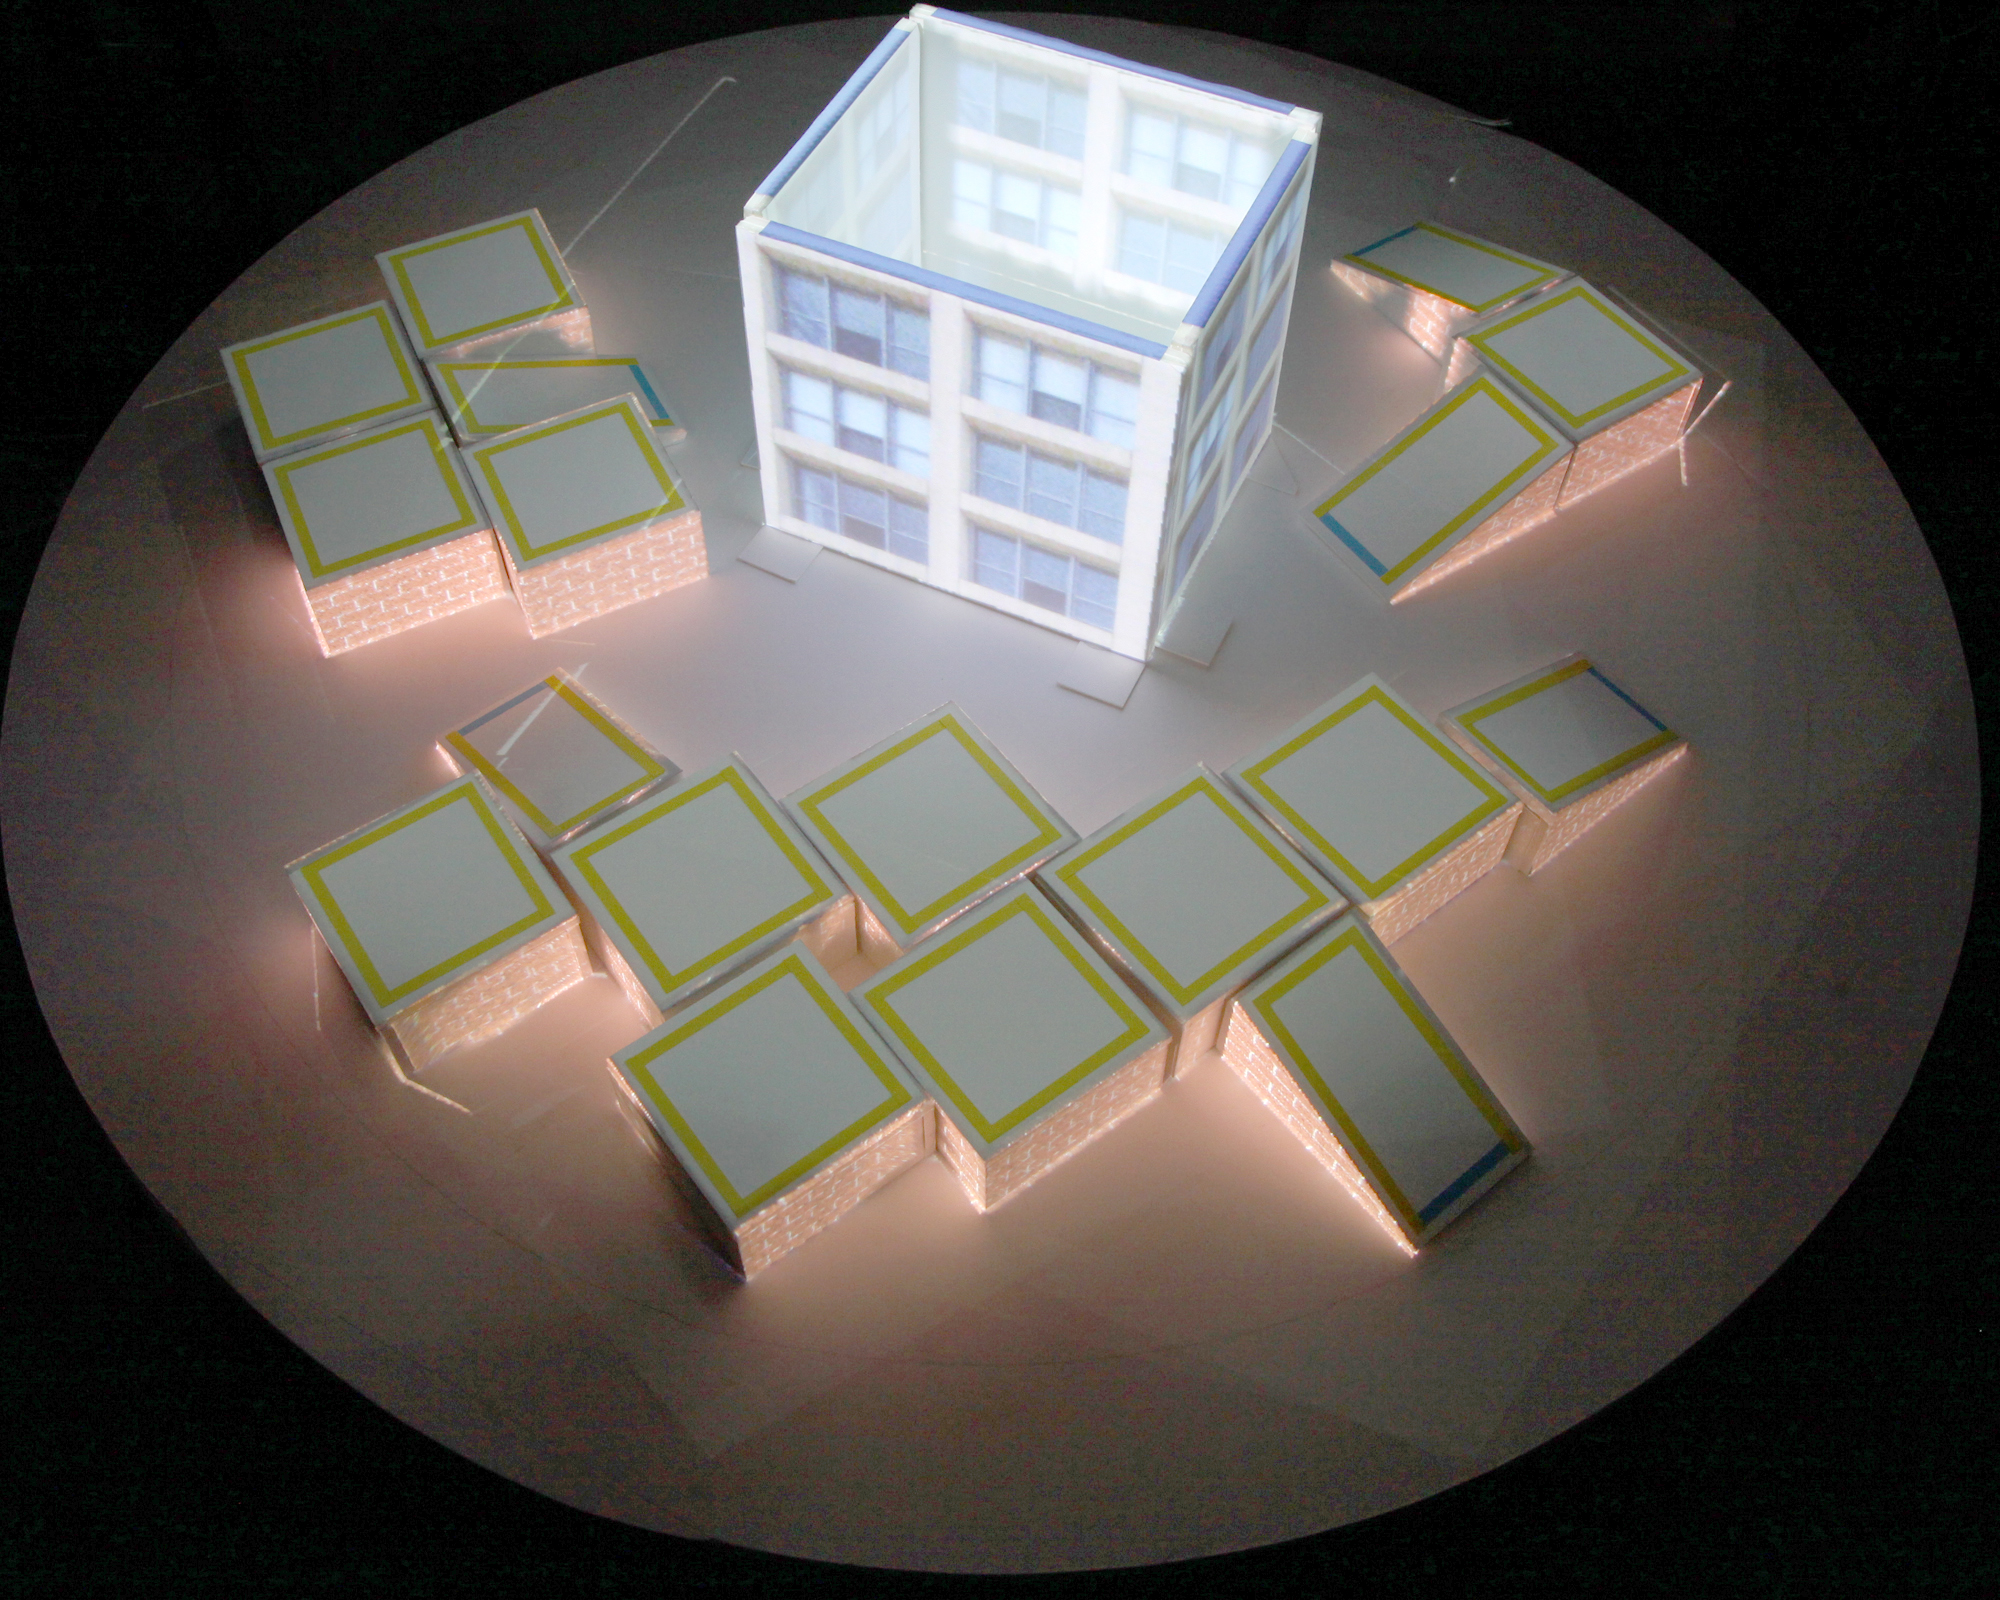
\includegraphics{images/complex_projection_lightened.jpg}}%
\vspace{-0.1in}
\caption[Terrain Placement]{Players freely arrange platform, ramp, and
  wall terrain objects in the scene, and our system detects and
  augments these objects with appropriate and interesting textures. }
\label{FIGURE:TerrainPlacement}
\end{figure}


%% An important aspect of many tabletop games, particularly those that %% involve military strategy, is the idea that the game world is not flat %% and uniform, but rather that it is characterized by varying terrain.  %% As in the real world, terrain represents variations in elevation and %% environment that affect units within the area.  For example, one kind %% of terrain might represent a swamp that is difficult to walk through, %% resulting in a movement penalty to units attempting to move through %% the terrain.  Another might represent tall grass that provides some %% degree of cover, thus making it more difficult to fire at concealed %% units in combat.  

%Walls represent tall barriers through which units cannot move or see.  %Elevated platforms serve a similar function, but differ in that units %may stand and move around on top of them.  

Like most miniature war games, ARmy is played on a varied 3D terrain
surface requiring strategic decision making. The ARmy prototype
provides three simple terrain object types: 8'' vertical walls,
elevated platforms (4'' x 4'' x 2'' high), and ramps (3'' x 5'' x 2'' high).
Units are not allowed to ``jump'' or ``climb'' from low elevation to
high elevation or vice versa, but must instead use connected ramps
to walk between the two.  Controlling elevated terrain and
ramps is important to the strategy of the game, as units that hold the
higher ground receive a significant advantage in combat.

%An appealing aspect of ARmy is that, like most miniature war games, %it allows players to be creative in their construction of the game %world, designing the terrain configuration to suit strategies that %seem fun and exciting.  
%% Figure~\ref{FIGURE:GamePrimitives} shows a representative set of %% object types that are used in the game.  Wall primitives are 8'' tall %% by \begin{math}\frac{1}{2}\end{math}'' thick, and are available in a %% variety of lengths.  Elevated terrain is composed of 4'' long by 4'' %% wide by 2'' tall platform primitives, as well as 5'' long by 3'' wide %% ramp primitives.

The game begins with a \emph{terrain placement} step, during which
players decide on the terrain layout by freely placing provided
terrain primitives on the table
(Figure~\ref{FIGURE:TerrainPlacement}).  Each primitive is constructed
from diffuse white foam-core with simple unobtrusive colored markings
to facilitate detection.  To simplify the game rules as well as the
task of detecting the terrain, we require that platforms and ramps
will not be stacked on top of each other, and that terrain placement
will not change after the game has begun.  After both players have
agreed upon an acceptable terrain configuration, they 
signal the application, which locks their decision.


%% In traditional miniature war games, players are typically allowed to %% represent terrain using whatever objects or methods may be available %% to them.  However, many players prefer to use objects that physically %% resemble the terrain that they represent in order to make it easier %% for players to remember the meaning of each object.  In addition, %% realistic terrain objects help to create a more aesthetically sound %% environment, which may help some players to feel immersed in the %% miniature world of the game.  In this regard, techniques for spatial %% augmentation hold great promise as a means of flexibly applying a wide %% number of aesthetic choices to a single primitive object.

The ARmy application uses the underlying SAR projection system to
apply virtual textures directly onto the physical terrain primitives.
Figure~\ref{FIGURE:TerrainPlacement} shows an example terrain
configuration with and without augmentation.  Brick textures are
applied to the sides of elevated ramp and platform terrain, and a
windowed building facade texture is applied to the wall surfaces
%.  Of
%course, these textures are merely an example of one possible aesthetic
%choice, and could easily be replaced with anything desired by the
%players, such as grass, concrete, or sandbags.

%% It is important to note that many players of miniature war games enjoy %% constructing and customizing terrain objects as much as they enjoy %% playing the game itself.  For this reason, an ideal application of %% spatially augmented reality would not prohibit players from crafting %% and using such objects.  In other words, visual augmentation is not %% intended to replace fine craftsmanship, but instead to be available %% only when players desire it.  For example, consider a situation in %% which a player wishes to make last-minute changes to a setup, thus %% requiring him to add primitive objects to an otherwise highly-detailed %% scene.  In this case, projecting a few well-chosen textures can help %% maintain the visual integrity of the game.


\subsection{Army Placement}

After configuring the terrain, players decide on rules for positioning
their respective armies.  Units are represented using 2'' tall plastic
soldier figurines, which have been colored with red or green spray
paint to denote player ownership.  As in any figurine-based tabletop
game, units are positioned by physically placing them on the table.
At any point during this step, players may request an update from the
game module, which will then detect all positioned figurines, marking
each with a colorful projected icon to show that it has been
successfully recognized.
%, as depicted in
%Figure~\ref{FIGURE:CombatMovementExample}b.  
When all units have been placed to the players' satisfaction, they
signal for the game to start.


\begin{figure*}[t]
\newcommand{\picwidth}{1.14in}
\resizebox{\picwidth}{!}{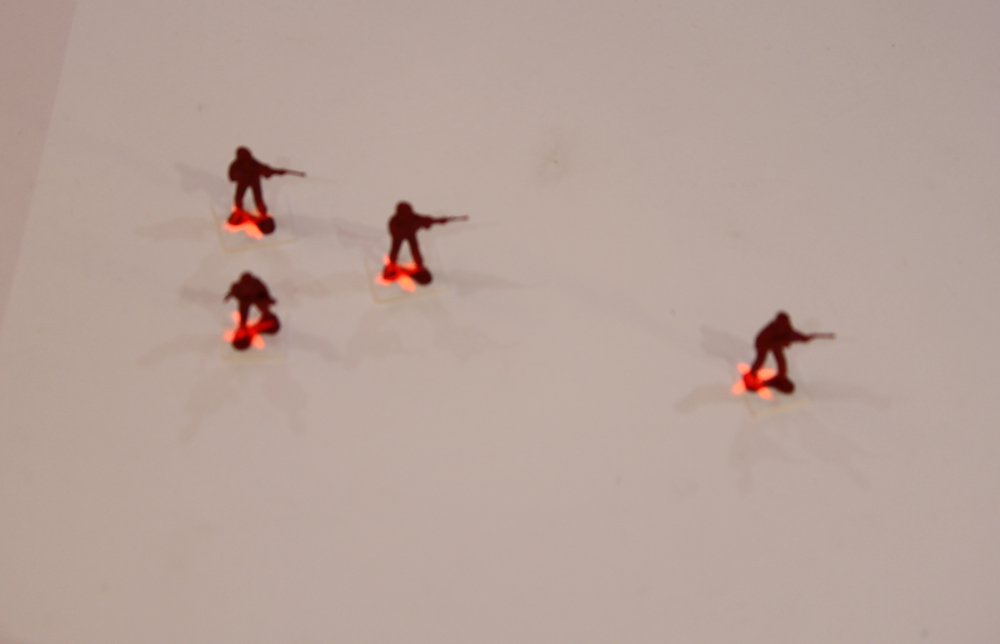
\includegraphics{images/movement_0.jpg}}
\resizebox{\picwidth}{!}{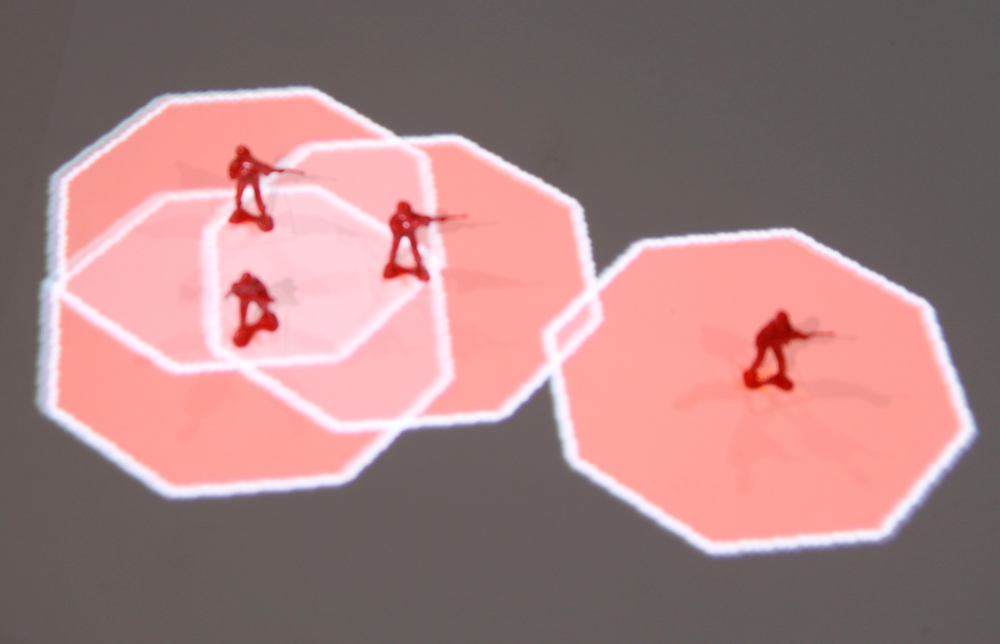
\includegraphics{images/movement_1.jpg}}
\resizebox{\picwidth}{!}{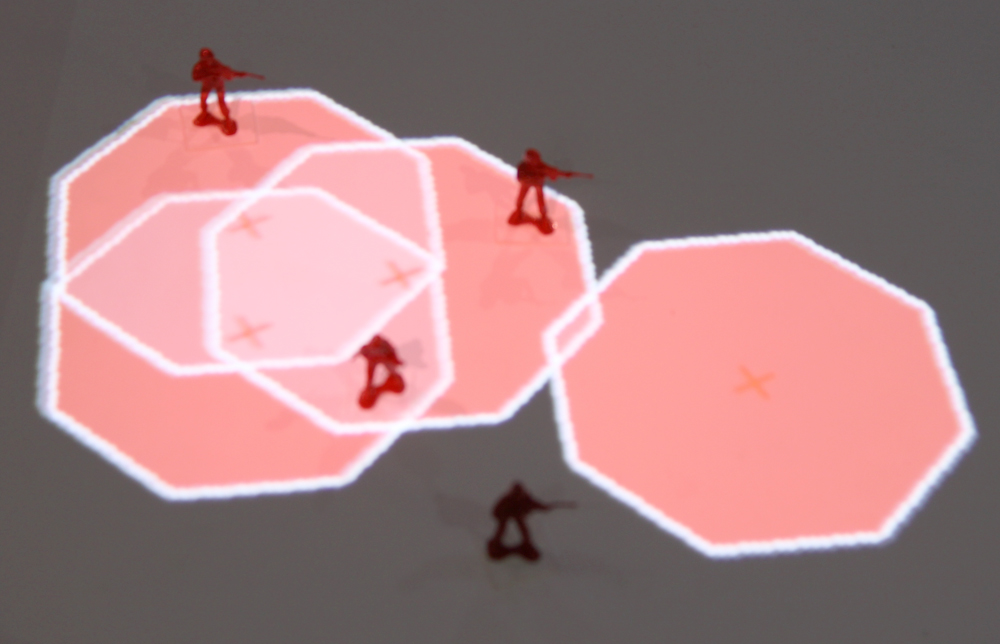
\includegraphics{images/movement_2.jpg}}
\resizebox{\picwidth}{!}{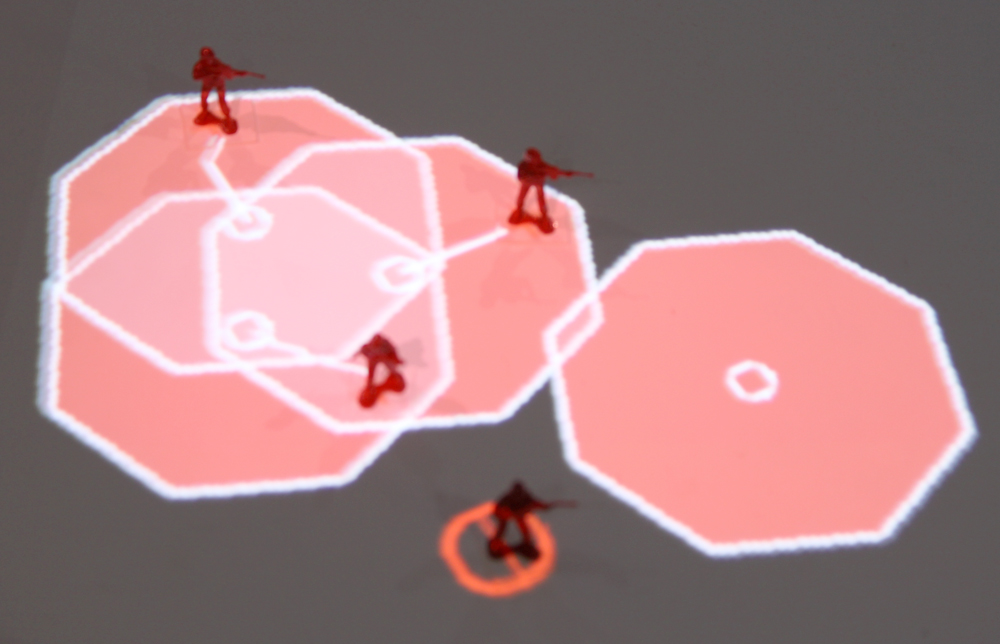
\includegraphics{images/movement_3.jpg}}
\resizebox{\picwidth}{!}{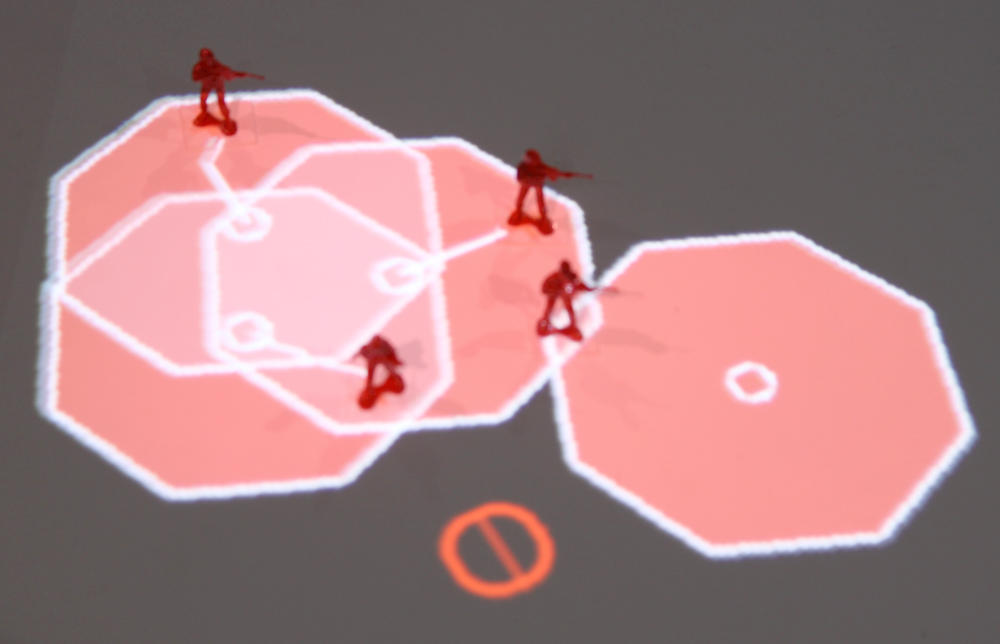
\includegraphics{images/movement_4.jpg}}
\resizebox{\picwidth}{!}{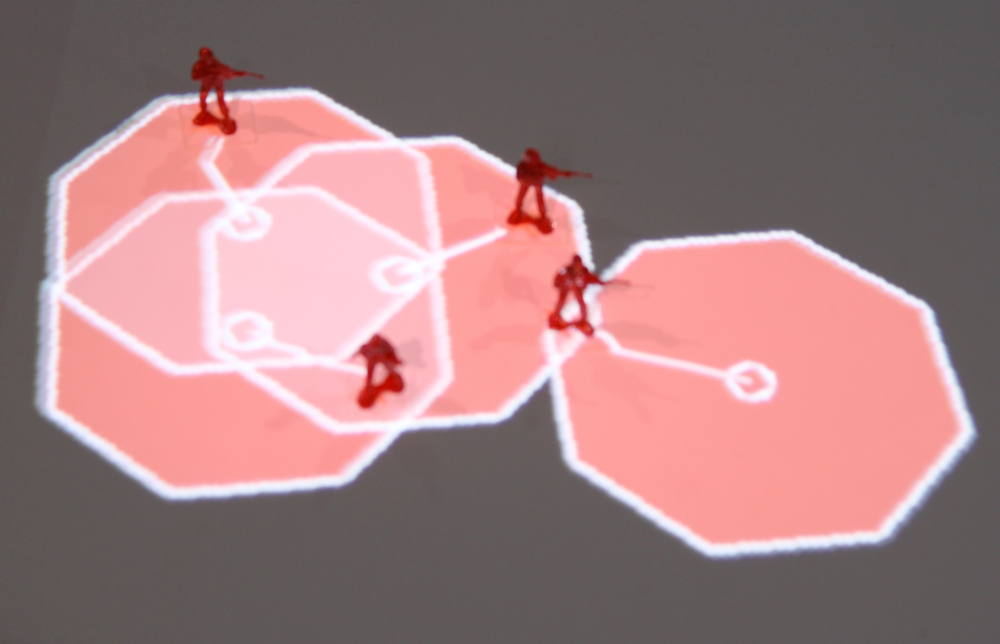
\includegraphics{images/movement_5.jpg}}%
\vspace{-0.1in}
\caption{During each movement phase the player may move all of their
  units simultaneously.  The system matches each unit's current
  position to the last known position using the Hungarian Method
  (marked with white paths).  If no legal move is found the unit is
  marked appropriately.  The player must then correct the error.
}
\vspace{-0.15in}
\label{FIGURE:MovementSequence}
\end{figure*}



\subsection{Movement Phase}

Each player's turn consists of a \emph{movement phase}, during which
he has the option of moving any number of his units.  As in most
tabletop war games, a unit's movement is constrained to a specified
distance (4'' for our game), and must conform to the movement rules
dictated by the terrain.
%
In the traditional, non-augmented version of this type of  game,
%er, a crucial difference is that in a traditional game, 
players are required to measure distances using a ruler or measuring
tape.
% to make sure that all moves fall within the acceptable range.  
%
%As
%previously stated, 
Augmentation is helpful
%one goal of augmenting physical games with elements
%of video games is to
in automating tedious tasks
% that would otherwise burden the player, as
as well as subjective calls that could lead to disagreements between
players about the legality of specific moves.  In the augmented
version of the game,
%In this case, the game module completely eliminates the
the system 
%need for players to manually measure distances by 
clearly and precisely indicates each unit's field of movement, and
reduces ambiguity in rules by notifying players when a move is
illegal.  Additionally, since players may move many units at once, the
augmentation keeps track of which units have already been moved from
their initial positions, thereby avoiding a potential source of
confusion.

% FIGURE OF EXAMPLE MOVEMENT REGIONS
\begin{figure}[b]
\newcommand{\picwidth}{1.65in}
\resizebox{\picwidth}{!}{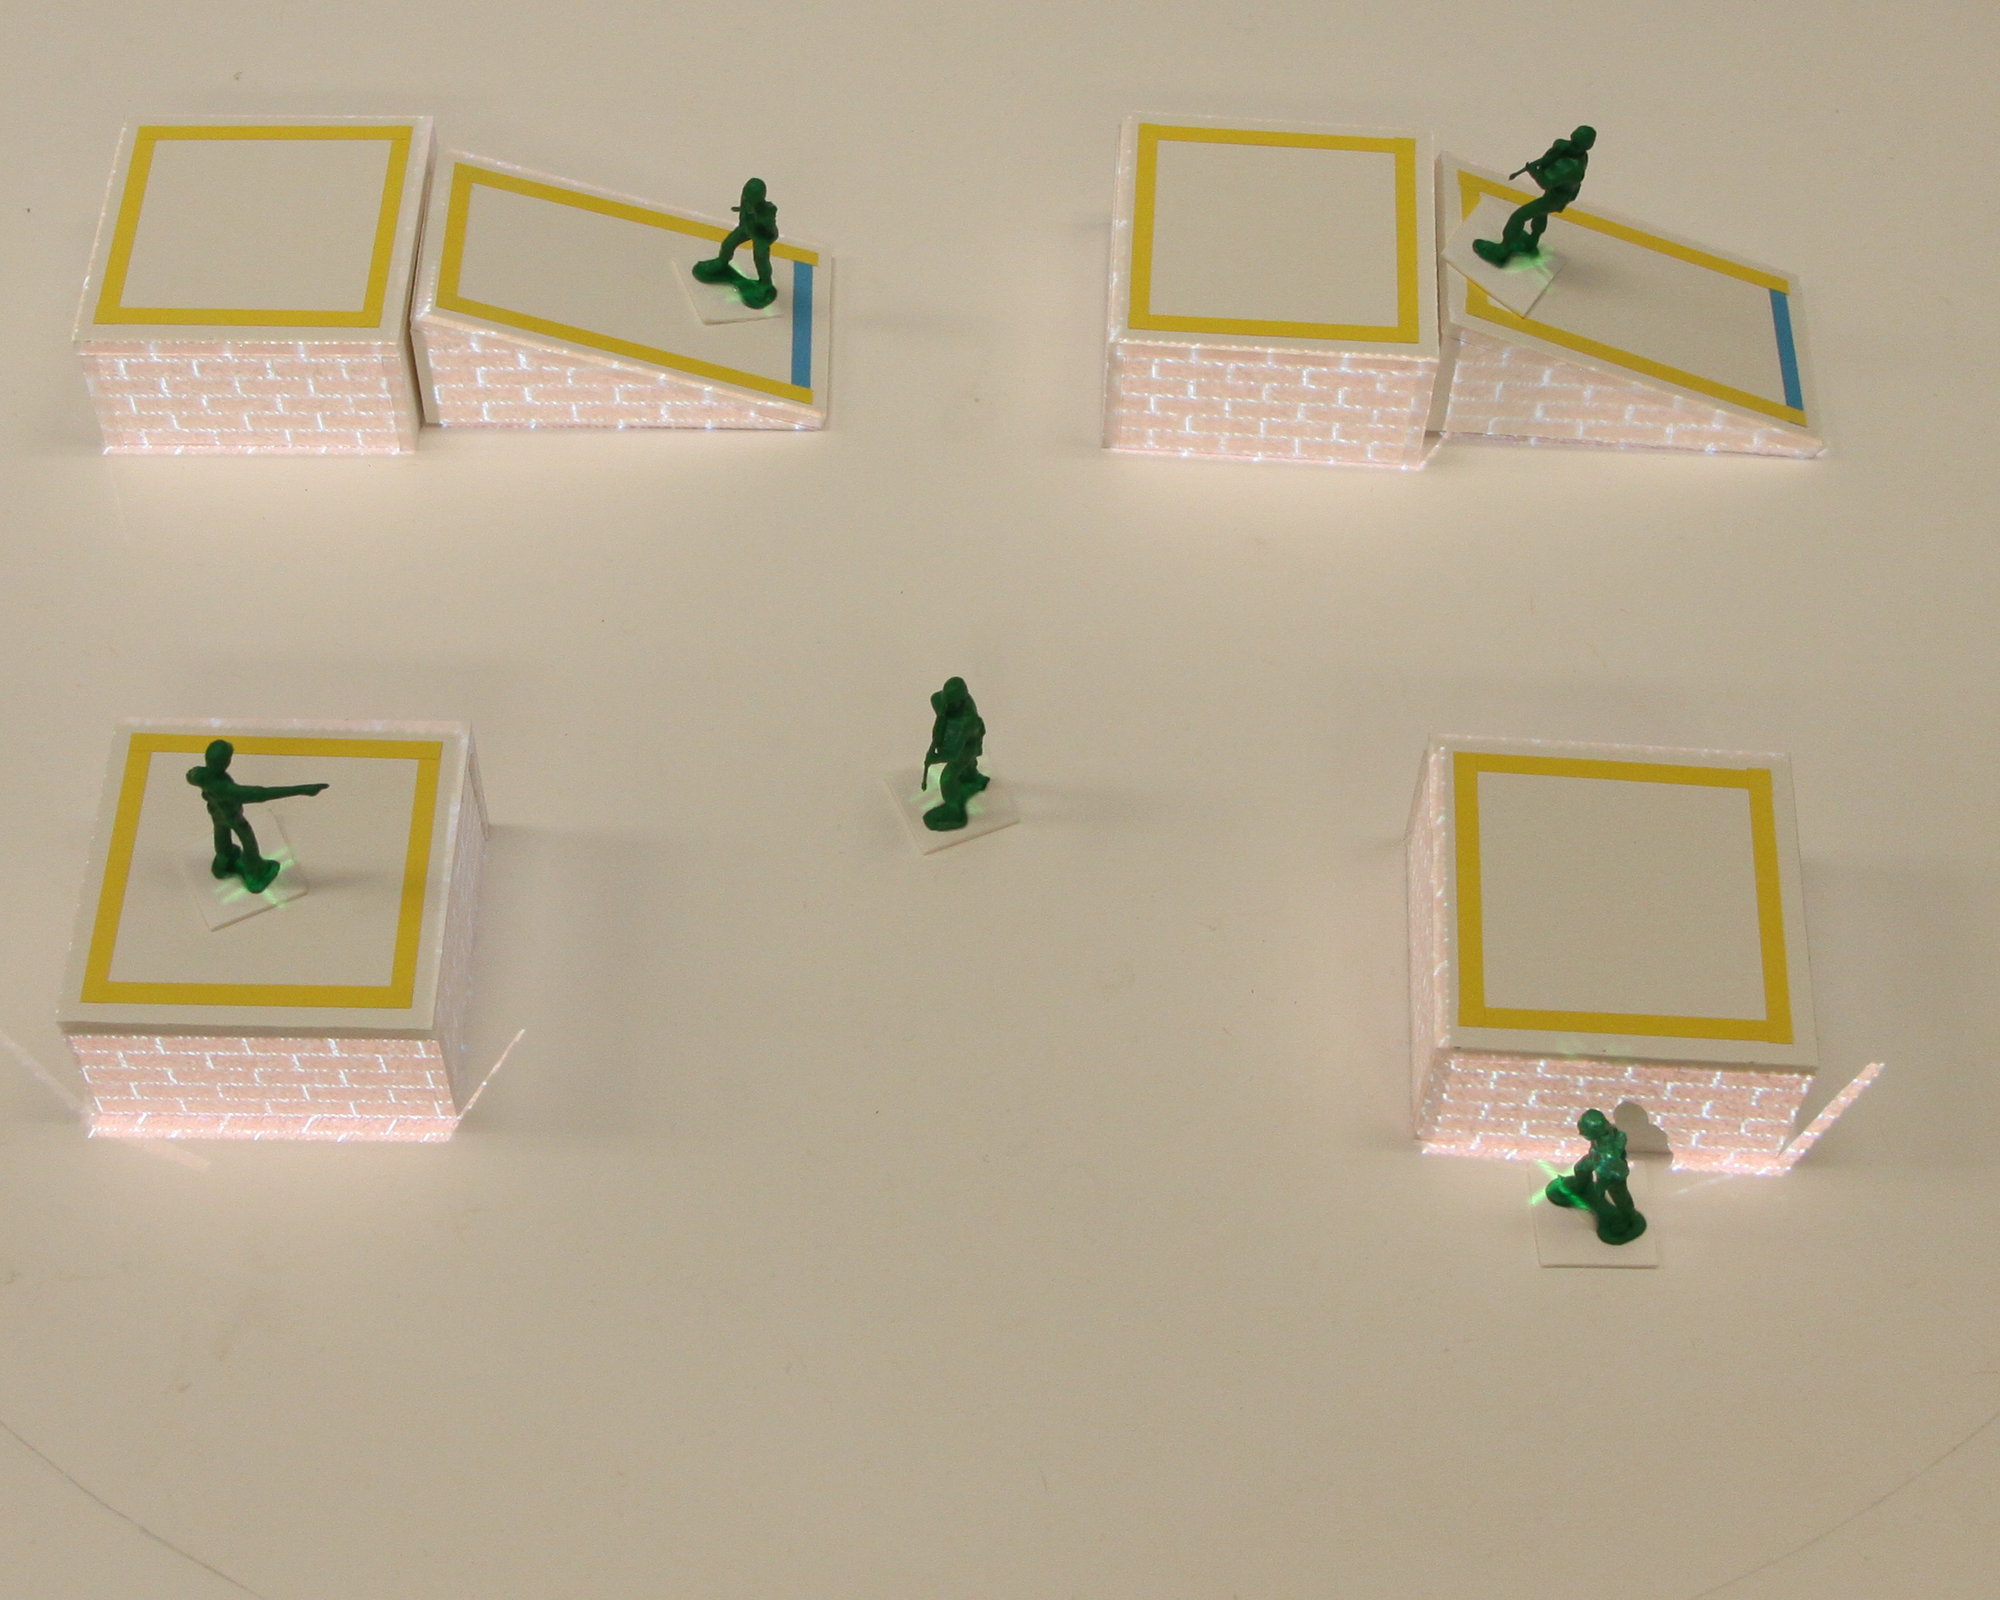
\includegraphics{images/movement_terrain_projection_lights_on_with_army.jpg}}
\resizebox{\picwidth}{!}{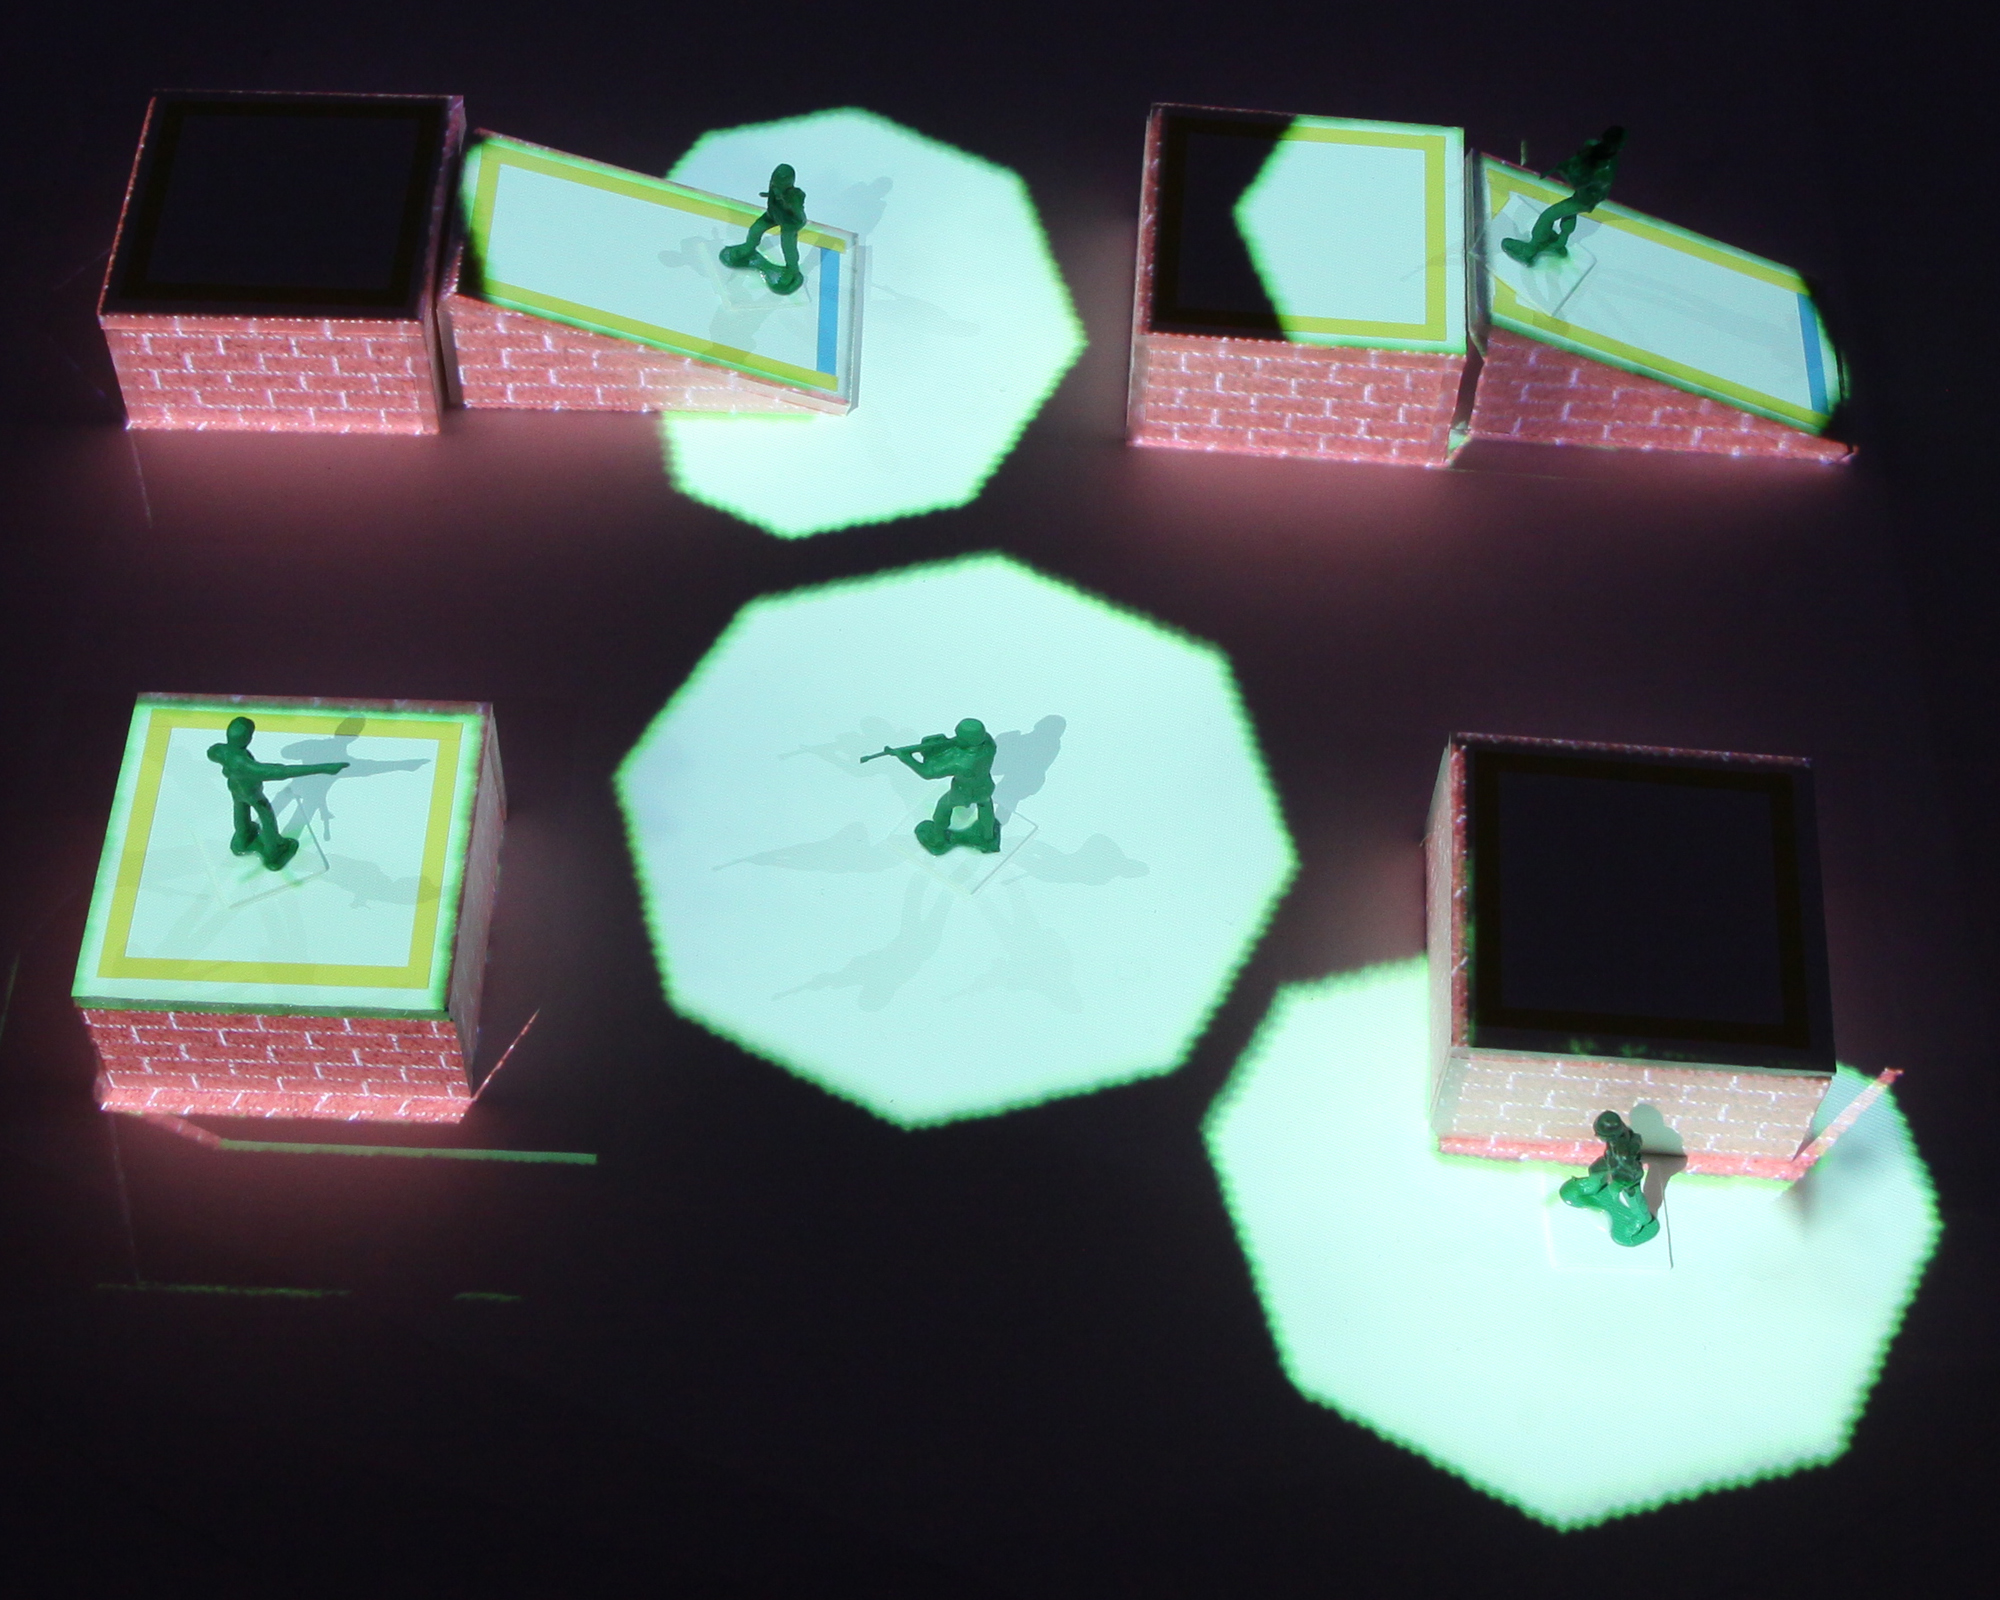
\includegraphics{images/movement_circles_projection.jpg}}%
\vspace{-0.1in}
\caption{During a player's \emph{movement phase,} each unit's field of
  movement (limited to 4'') is illuminated.  Note that each unit's
  movement field accounts for movement rules across terrain
  boundaries, which require the use of ramp objects in order to climb
  up or down elevated platform.  }
\label{FIGURE:MovementRegions}
\vspace{-0.1in}
\end{figure}






At the start of the movement phase, each unit's field of movement is
overlaid on the terrain as a colored region 
%\fbox{repetitive? perhaps switch the order of paragraphs?}
(Figure~\ref{FIGURE:MovementRegions}).  The player may move the unit
anywhere within its corresponding highlighted region.  At any point
during the movement phase, the player may request an update of the
visualization from the game module.
%, which will then augment the
%overlayed display with a visualization of the desired moves.  
Each unit's position at the start of the movement phase is denoted by
a ``$\circ$'' icon and its current position is marked with an an
``$\times$'' icon with a white line connecting the positions, marking
the unit's movement path (Figure~\ref{FIGURE:MovementSequence}).
In the event that a given move is invalid, this information is
reflected in the overlay, allowing the player to correct the error.
The game continues to display the movement zones of each unit from its
original position, in case the player changes his mind and would like
to choose a different move for a particular unit.

\subsection{Combat Simulation}
\label{SECTION:CombatSimulation}


\begin{figure}[b]
\newcommand{\picwidth}{1.65in}
\resizebox{\picwidth}{!}{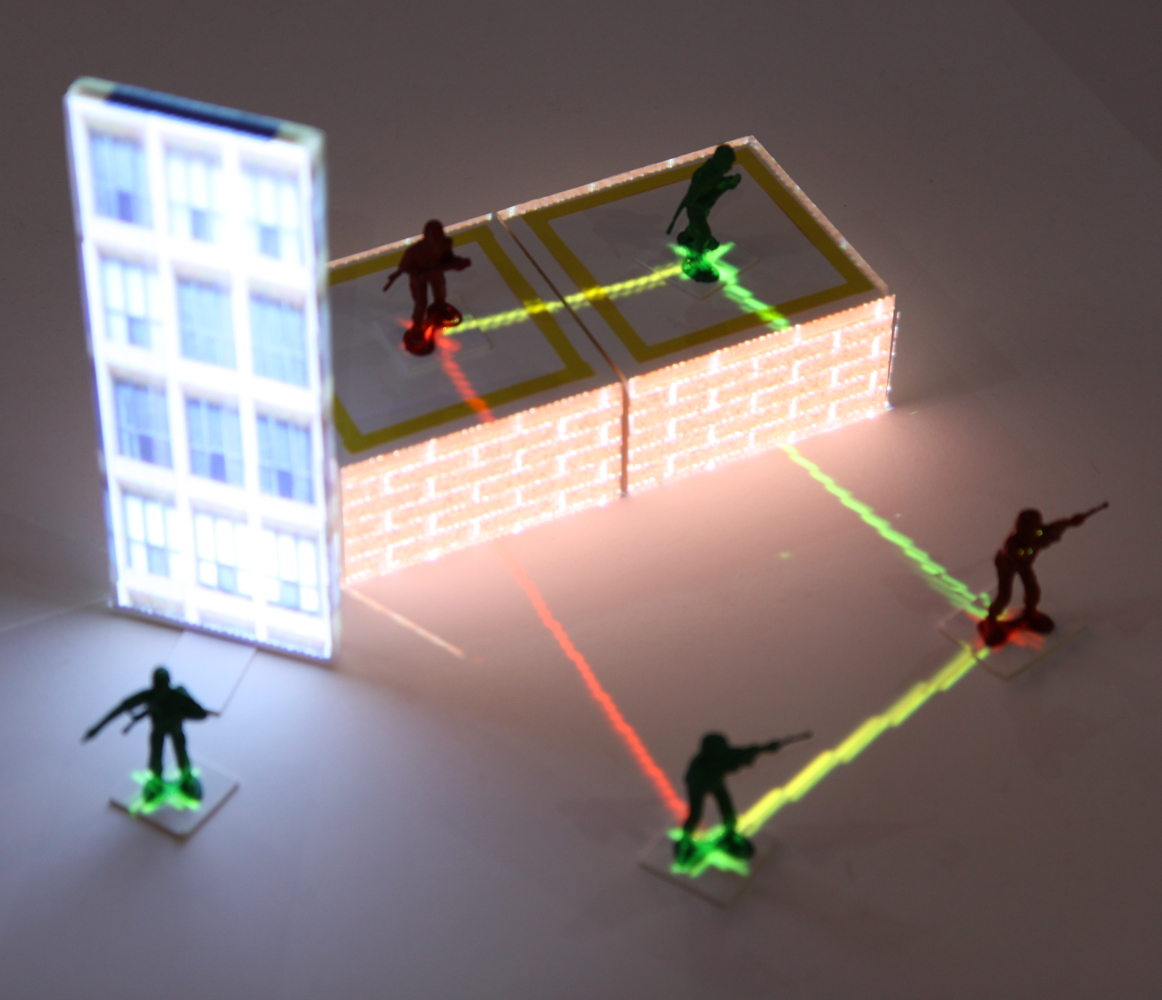
\includegraphics{images/combat_image_b.jpg}}
\resizebox{\picwidth}{!}{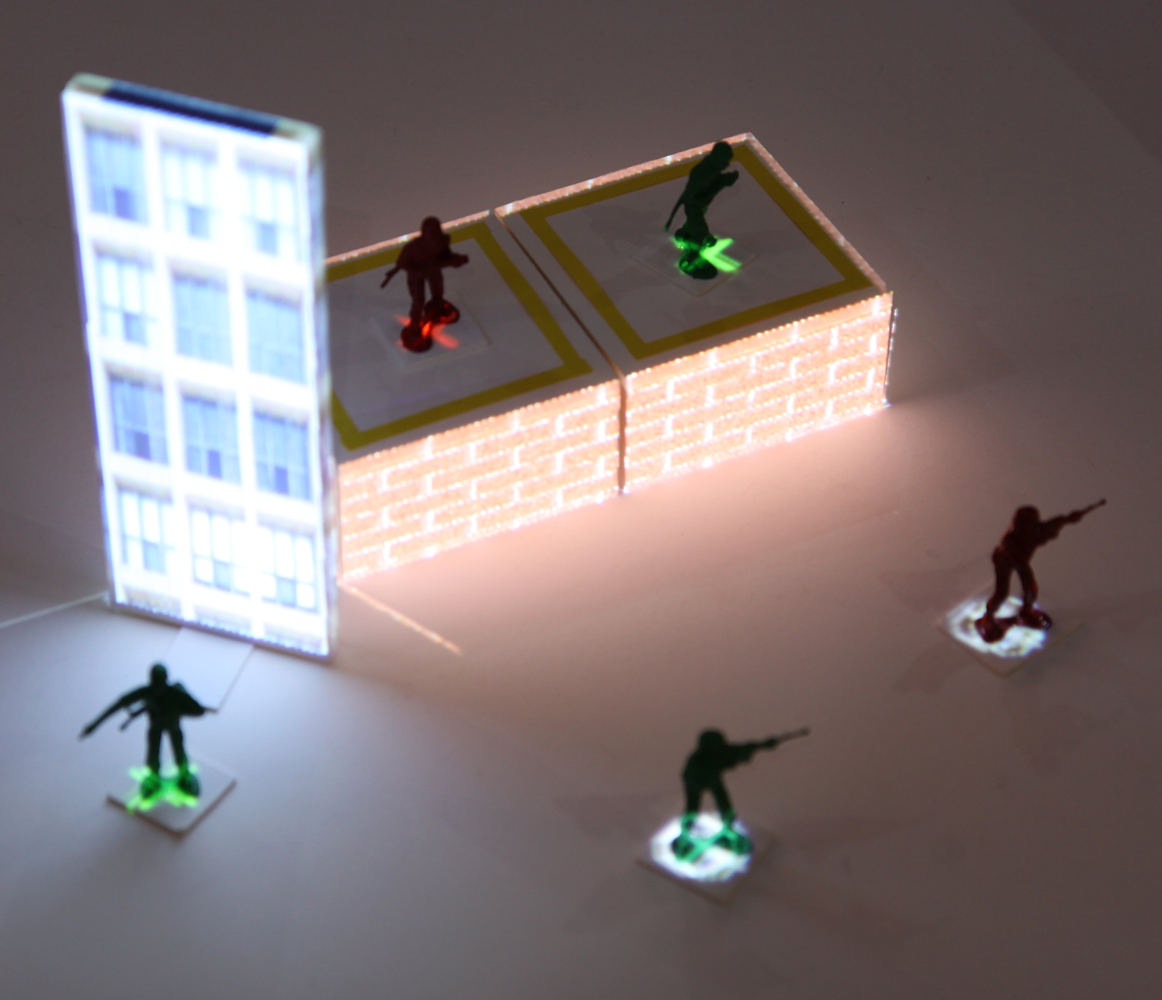
\includegraphics{images/combat_image_c.jpg}}%
\vspace{-0.1in}
\caption{Brightly colored {\em combat lines} indicate which units are
  within firing range and have a {\em line of sight} to an opposing
  unit.  Yellow lines indicate combat between units on equal height.
  A red line indicates a height advantage for the red player and
  similarly a green line indicates a height advantage for the green
  player.  Note that the leftmost green unit's line of sight to one
  red unit is blocked by the wall and the other red unit is more than
  8 inches away.  After the combat round, two units are marked for
  removal.  }
\label{FIGURE:CombatExamples}
\end{figure}


%% In addition to moving about the game world, tabletop war games require %% that units be able to engage other units in combat.  Generally %% speaking, combat occurs when one player uses a particular unit to %% initiate an attack on an opposing unit.  A unit that receives too many %% successful attacks is defeated and usually must be removed from play.  %% Typically an attack can only be carried out across a specified %% distance range, and sometimes also requires that the attacker be able %% to ``see'' the target.  In order to check that a valid line of sight %% exists between the two units, players often must crouch or lean over %% the table, align their eyes with the attacking figurine's ``point of %% view,'' and verify that the target figurine is visible and %% unobstructed by terrain or other objects.  After a valid attack has %% been declared, its effectiveness is determined according to combat %% rules, which often involve rolling dice.  Once again, all of these %% tasks represent prime opportunities for automation.

The current game prototype handles combat in a different manner from
typical miniature war games, in that attacks are not explicitly
declared by the players.  Instead, each movement phase is followed by
a \emph{combat simulation round}, during which all units automatically
attack available targets in a range of 8 inches.  This is somewhat
more similar to how combat works in a typical real-time strategy (RTS)
video game, in which individual ``smart'' units exhibit a certain
amount of autonomy in their actions, following orders only to the
extent allowable by their preprogrammed behaviors.
%
%% The idea of commanding ``smart'' units in combat interactions is not %% something that can be practically simulated by traditional tabletop %% war games, but is an interesting possibility for augmented reality %% games like ARmy.
%
As players move units around the battlefield, colored ``combat line''
visualizations are overlaid on the ground textures, connecting
opposing units that are able to attack each other
(Figure~\ref{FIGURE:CombatExamples}).  This visualization provides
important feedback to help players plan moves strategically.  During a
subsequent combat round, the game module iterates through all such
connected pairs and in each case simulates an individual contest,
which may result in one or both units being eliminated.  In our game,
a unit on equal or lower ground than an opposing unit has a $1/3$
chance of disabling the opposing unit. A unit on higher ground
than the opponent has a $2/3$ chance of disabling the opponent. In a
non-augmented game, this is determined by rolling a 6-sided die.  At
the end of the combat simulation round, units that have been
eliminated are marked with a white ``$\otimes$'' icon, signaling to
the players that these figurines should be removed from play.  Once
all eliminated units have been correctly removed, the players signal
for the game to continue into the next movement phase.

\section{Implementation Details}
%% \section{System Overview}

%% Although our small-scale and large-scale systems differ in a number of %% ways, the two can be understood as variations of a single design, %% divided into a number of components.  The purpose of this section is to %% provide a high-level outline of this system, describing the role of %% each individual component.

%% An important principle of the general system design is that each %% component represents a single autonomous process.  Since the various %% responsibilities of a given component may require it to run at %% different rates than others, we decouple them such that at any point %% in time, a process can obtain the latest output from the previous %% stage of the pipeline (Figure~\ref{FIGURE:block_diagram}).  

%% \subsection{Camera Component for Scene Recognition and Tracking}

%% Projecting images onto a dynamic scene requires that our system be %% able to accurately recover the positions and orientations of objects %% and surfaces as they move.  We achieve this by tracking objects using %% images captured from a single camera mounted in an overhead position.  %% The camera hardware is capable of capturing and transmitting %% 1280\begin{math}\times\end{math}960 pixel images through a gigabit %% Ethernet connection at 33 frames per second.  Since the camera remains %% stationary during system use, we recover both intrinsic and extrinsic %% calibration parameters as a precomputational step.  The small-scale %% system uses Zhang's method of calibration~\cite{Zhang2000}, while the %% large-scale system uses Scaramuzza's calibration %% model~\cite{Scaramuzza2006} for correcting distortion, since we equip %% the camera with a fisheye lens in order to increase the area of %% coverage.

%% \subsection{Vision Component }

%% The \emph{vision component} is responsible for processing the raw %% camera output in order to achieve 3D registration of objects in the %% scene.  Of all the system components, the vision module is the one that %% differs most between the two system variants.  Because each system is %% built with different goals and constraints, each uses a completely %% different method for detecting objects.  In the large-scale system, we %% identify projection surfaces by tracking a number of embedded infrared %% LED markers, allowing us to ignore information in the visible light %% spectrum.  This is important because our large-scale system is built %% with the goal of achieving simultaneous acquisition and display to %% facilitate real-time applications.  In contrast, the small-scale system %% does not provide this feature, and instead detects objects using %% simple colored markers, making the objects lighter, cheaper, and %% easier to construct.  In either case, the output of the vision module %% is a list of detected objects and associated positional data, which we %% refer to as the ``skeleton geometry'' of the scene.

%% \subsection{World Modeling Component }

%% Skeleton geometry alone generally does not provide a sufficient %% representation of the scene for augmentation.  Instead, this %% information is passed to the \emph{world modeling component}, which is %% responsible for constructing a more complete environment model in %% order to suit the needs of the rendering modules, and sometimes the %% application.  The output is a three-dimensional virtual model of the %% scene in the form of a triangle mesh.  Additionally, two-dimensional %% heightfield representations of the scene can be provided if needed by %% a particular application.  
%% %Additionally, this module uses projector calibration data to compute %% %a set of blending weights used to smooth variations in intensity %% %across regions of projector overlap.

%% \subsection{Display Controller and Projector Renderers }

%% Because the number of projectors that a particular machine may drive %% is limited to the number DVI output ports that it provides, our system %% uses a distributive rendering process to divide the workload across %% multiple computers.  Our most recent configuration is capable of %% driving a maximum of eight projectors by using two servers, each %% equipped with two dual-head graphics cards.  We accomplish this using a %% single \emph{display controller,} which coordinates a number of remote %% \emph{projector renderer} modules.  The display controller sends %% relevant display information to the separate renderers, including the %% geometric model and textures.  Each projector renderer controls the %% display of a single projector and generates the final display image by %% rendering the virtual model of the scene from the perspective of the %% projector based on calibration data.

The ARmy application was built on top of a multi-projector SAR system.
This section explains in greater detail the ways in which the
application interacts with the underlying system modules, as well as
the algorithms used to perform various game operations.

\subsection{Object Detection }

%FIGURE : Object detection images

\begin{figure*}[t]
\begin{center}
\newcommand{\picwidth}{1.72in}
 \resizebox{!}{\picwidth}{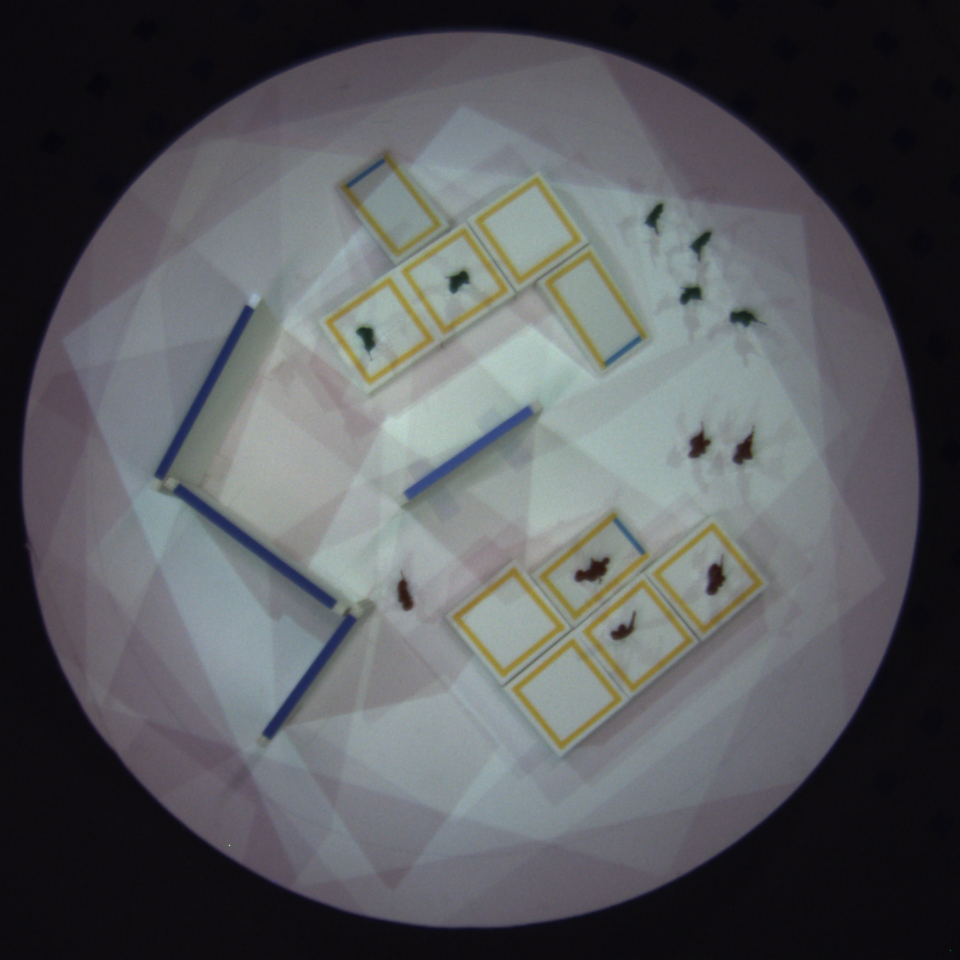
\includegraphics{images/raw_with_soldiers.png}}
 \resizebox{!}{\picwidth}{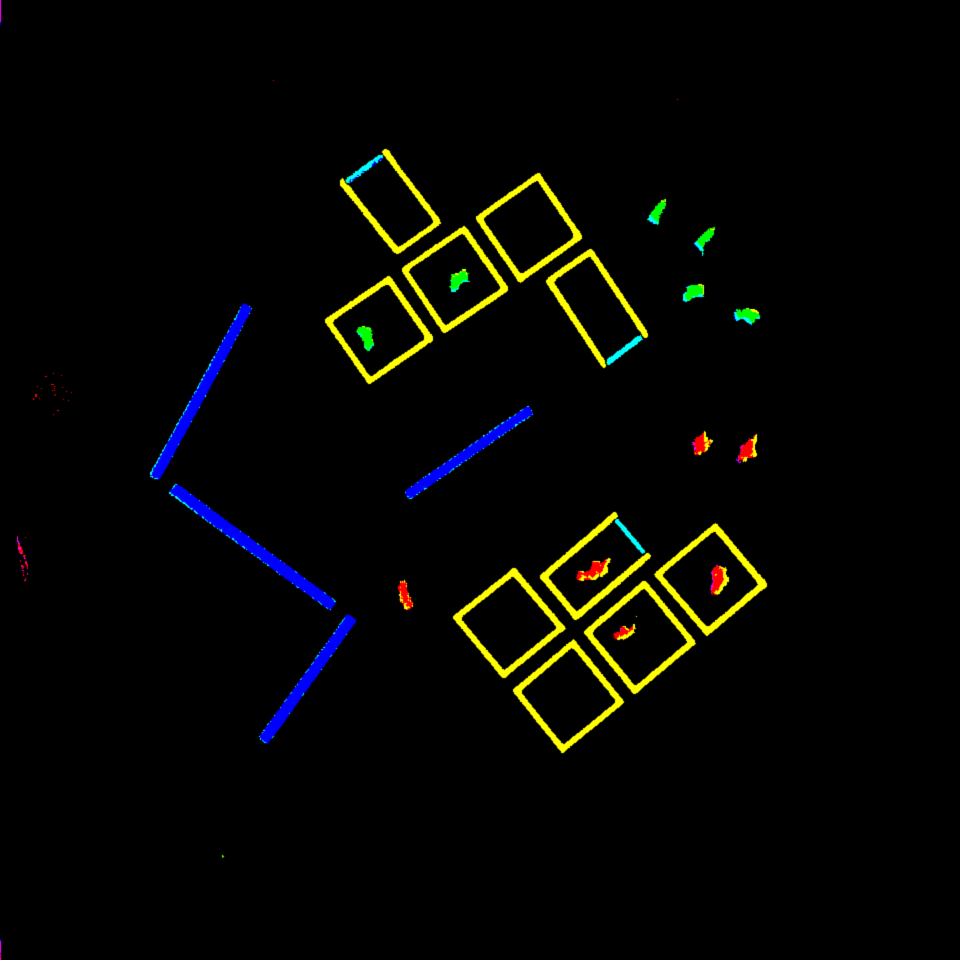
\includegraphics{images/enh_colors_with_soldiers_blur.png}}
 \resizebox{!}{\picwidth}{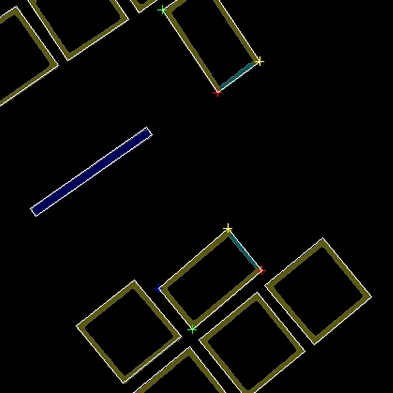
\includegraphics{images/terrain_labels_crop.png}}
 \resizebox{!}{\picwidth}{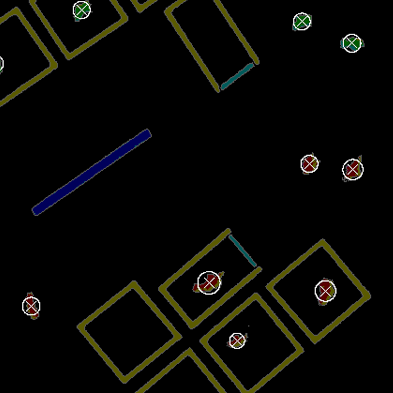
\includegraphics{images/labels_with_soldiers_crop.png}}\vspace{-0.2in}\\
\begin{minipage}{\picwidth}\textcolor[rgb]{1,1,1}{\hspace{0.02in} {\bf        a)}} \end{minipage}
 \begin{minipage}{\picwidth}\textcolor[rgb]{1,1,1}{\hspace{0.02in} {\bf        b)}} \end{minipage}
 \begin{minipage}{\picwidth}\textcolor[rgb]{1,1,1}{\hspace{0.02in} {\bf              c)}} \end{minipage}
 \begin{minipage}{\picwidth}\textcolor[rgb]{1,1,1}{\hspace{0.02in} {\bf              d)}} \end{minipage}
\end{center}
\vspace{-0.15in}
\caption[ARmy Object Detection]{a) Raw camera images of the scene show
  variable lighting due to shadows and regions of projector overlap.
  The \emph{vision component} ignores these artifacts by considering
  b) only pixels with highly saturated color properties, which it
  groups into connected components. These components are classified as
  c) quadrilateral terrain regions or d) soldier figurines based on
  size, color, and shape.}
\label{FIGURE:ARmyObjectDetection}
\vspace{-0.1in}
\end{figure*}

%Our SAR tabletop system detects objects using a single calibrated %camera mounted overhead for a top-down viewpoint.  
During acquisition, a single image from the overhead camera
(Figure~\ref{FIGURE:ARmyObjectDetection}) is processed by our vision
module, which uses thresholding techniques to identify connected image
components with predominant color attributes matching a set of
identifiable colors. 
% Currently the set is limited to a six color
%vocabulary, including red, green, blue, yellow, cyan, and magenta,
%which has proven sufficient for a number of applications developed
%using the system.
%
%Because the game is designed with the assumption that terrain does %not change beyond the initial setup phase, which occurs before %soldier units have been placed in the scene, the classification rules %can be separated into two distinct sets, allowing the vision module %to operate in separate modes.
%
After a colored component is detected, the vision module attempts to
classify it as one of the known game object primitives.  During the
terrain placement phase, the system detects the initial configuration
of terrain objects, which are encoded with the colors blue, yellow,
and cyan.  Blue components that fit a rectangular shape within an
acceptable margin of error are classified as wall objects.  Platform
objects are detected in the image as yellow components with a valid
quadrilateral fit.  Similarly, ramps are classified from quadrilateral
components with three predominantly yellow sides and one predominantly
cyan side.  The cyan side indicates the low edge of the ramp, which
reaches down to the table surface.  Once an appropriate quadrilateral
has been fit to a terrain object, the corners are used to specify
position and orientation.

After the terrain setup has been finalized, subsequent scene
recognition steps use the second detection mode, which is responsible
for identifying soldiers.  Since red and green colors are reserved for
soldier figurines, any appropriately sized red or green component 
%that falls within an
%acceptable range of sizes 
is classified as a soldier unit.  Each detected unit is assigned a
single location equal to the centroid of the component in image space.

Once a component has been classified as a valid object, its known
world dimensions are used in combination with the calibration data of
the camera to determine its position and orientation in world space.
Calibration of the camera and the projectors is performed as a
preprocessing step~\cite{Zhang2000}.  Overall,
our color-based detection method successfully and robustly recognizes
a variety of objects without the need for large fiducial markers or
embedded sensors, allowing us to easily construct a sizeable
collection of simple objects.

%% For any given pixel coordinates in the camera image, the calibration %% parameters define a ray in 3D space representing the corresponding %% path along which light enters the camera.  By using the known height of %% the object at that point, we can backproject along the ray to %% determine the exact world position.

%%  Objects with natural color %% properties, such as brightly colored game pieces, can often be tracked %% without any modification, while objects that lack these properties can %% be tracked with the simple addition of colored markers.

%\subsection{ Virtual Modelling of the Scene}

%As discussed in the system overview, our \emph{world modelling} %component is capable of constructing both 2D and 3D virtual %representations of the physical scene.  The ARmy game application uses

%In order for our system to dynamically project on the detected %objects, it is necessary that we compute a virtual model of the %scene.  This step is handled by a different system component, which %receives the positional data of the detected objects and outputs a %three-dimensional mesh that closely matches the real-world geometry.  %In addition, this module is capable of outputting a two-dimensional %heightfield of the scene, a feature that is utilized by the ARmy game %in order to obtain a simplified representation of the game world.

%\fbox{Mention texture stuff here? Special-case UVs for floor?} \\
%\fbox{Also, does it sound like I'm taking credit for this?}

\subsection{Modeling the Game World }

%The game world is represented as a two-dimensional heightfield of the %scene, discretized into a high-resolution square grid.

Once the terrain objects have been acquired, the system computes a
two-dimensional heightfield representation of the scene.  This raw
heightfield is first processed to remove unwanted discontinuities,
such as small gaps between adjacent platforms and ramps that would
undesirably block the movement of units.  This is done by creating a
binary image from the heightfield, with foreground pixels representing
elevated terrain primitives.  Next binary dilation and erosion are
applied to the image, which fills in unwanted, narrow background
features.  The new foreground pixels are assigned reasonable height
values based on their neighbors (Figure~\ref{FIGURE:HeightfieldOperations}).

The modified heightfield is used to construct a connected movement
graph, which the game module uses to approximate the travel distances
of units as they move through the scene.  
%Each graph location stores
%the cost of moving from the cell to each of its eight neighbors,
%subject to a maximum height difference threshold.  
If the difference in height of two adjacent cells is below the
elevation difference threshold, then the cells are connect neighbors,
and the associated movement cost is equal to the Euclidean distance
between the two. 
%Otherwise the distance is set to infinity.\fbox{needed?}  
The
resulting graph reflects movements that are legal according to the
rules of the game, allowing for units to traverse flat terrain regions
and gradual elevation changes on ramps, but not to cross sharp
boundaries, such as cliffs or walls.  Because the terrain
configuration does not change after the terrain placement step, these
distance values are computed once at the beginning of the game.

%% Since each cell is connected to at most eight neighbors, the average %% size of the data per cell is invariant with respect to the number of %% cells in the grid, which means that this method scales reasonably to %% higher resolutions.

%% The result of this process is a connected graph that reflects the kind %% of movements expected according to the rules of the game.  Units may %% follow paths that traverse flat terrain regions, as well as ramps, %% which exhibit smooth height variations, but may not pass through sharp %% boundaries, such as cliffs and walls.  More complex movement rules %% could be integrated simply by changing the rules for assigning %% movement distances between neighbors.  For example, we could add a rule %% that soldiers move more slowly when walking up a ramp than when %% walking down one, by assigning costs asymmetrically between connected %% neighbors according to height differences.  The only requirement is a %% means of initializing the heightfield to accurately represent the %% terrain configuration constructed by the players.

%% As mentioned in the system overview, the world modeling component of %% our system is capable of providing a suitable heightfield rendering of %% the scene.  However, initializing the values of the grid from this raw %% heightfield output creates a few problems.  In fact, this height %% information is too accurate, in that it often captures tiny %% discontinuities that players would generally want to ignore.  For %% example, consider two platform objects that are placed side by side %% such that they are nearly touching, with the intention that units be %% able to move freely between the two.  Unfortunately, a thin crevice %% still exists between the two that is likely to be reflected in the raw %% heightfield.  If unaltered, this feature would result in an impassable %% barrier, defeating the intended purpose of the terrain configuration.

% FIGURE: HEIGHTFIELD OPERATIONS
\begin{figure*}[t]
\newcommand{\picwidth}{1.72in}
\begin{center}
 \resizebox{\picwidth}{!}{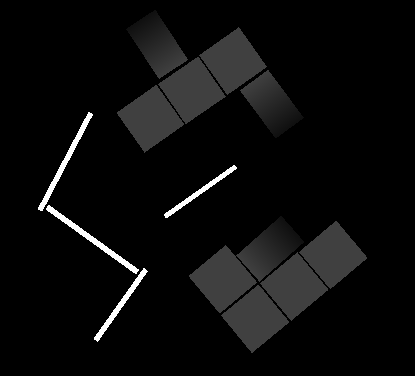
\includegraphics{images/initial_heightmap.png}}
% \resizebox{\picwidth}{!}{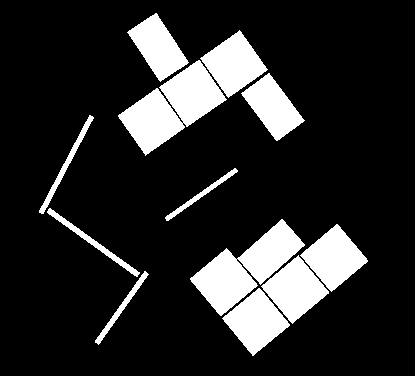
\includegraphics{images/floor_start.png}}
 \resizebox{\picwidth}{!}{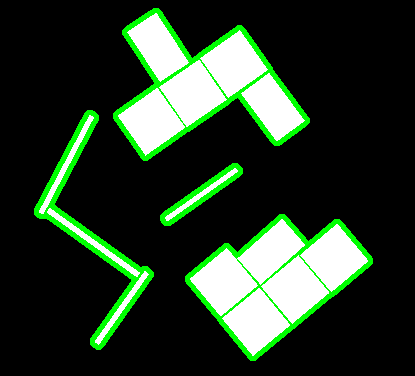
\includegraphics{images/floor_dilated_diff.png}}   %\vspace{-1.9in}\\
  \resizebox{\picwidth}{!}{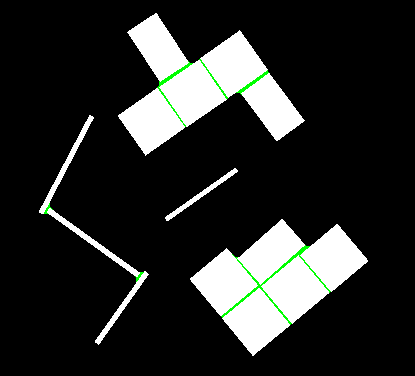
\includegraphics{images/floor_final_diff.png}}
  \resizebox{\picwidth}{!}{
\includegraphics{images/final_heightmap.png}}\vspace{-0.2in}\\

\begin{minipage}{\picwidth}\textcolor[rgb]{1,1,1}{\hspace{0.02in} {\bf        a)}} \end{minipage}
 \begin{minipage}{\picwidth}\textcolor[rgb]{1,1,1}{\hspace{0.02in} {\bf        b)}} \end{minipage}
 \begin{minipage}{\picwidth}\textcolor[rgb]{1,1,1}{\hspace{0.02in} {\bf              c)}} \end{minipage}
 \begin{minipage}{\picwidth}\textcolor[rgb]{1,1,1}{\hspace{0.02in} {\bf              d)}} \end{minipage}
 \end{center}
 \vspace{-0.15in}
 \caption[ARmy Game World Model]{The game world is constructed by
   beginning with an initial heightfield rendering of the scene (a)
   and filling in unwanted discontinuities.  
%First a threshold is
%   applied (b) to separate the floor from elevated terrain. 
 The next
   images show the results after dilation (b), and erosion (c), with
   green regions indicating differences from the original heightfield.
   These pixels are assigned new height values (d) to form the final,
   corrected heightfield.}
 \label{FIGURE:HeightfieldOperations}
\vspace{-0.1in}
 \end{figure*}

%% To solve this problem, I employ a few common image-space techniques to %% fill these unintended gaps.  The steps of this process are shown in %% Figure~\ref{FIGURE:HeightfieldOperations}.  First a threshold is %% applied to the heightfield, such that all pixels with height value %% greater than zero are set to the value of one.  The result is a binary %% image, in which all black background pixels correspond to the base %% height of the table surface, and all white foreground pixels %% correspond to terrain objects of higher elevation.  

%% Next I apply binary dilation and erosion, which in that order comprise %% an operation known in morphology as ``closing.'' Dilation involves %% centering an image kernel, in this case a disc, at each foreground %% pixel and activating the pixels that are overlapped.  This expands the %% foreground regions, filling in tight crevices and other undesired %% features.  Erosion performs another sweep with the same kernel, but %% instead deactivates locations where the kernel overlaps any background %% pixels.  This reduces the foreground components back to their %% approximate original size, but leaves the newly filled features %% intact.

%% Finally, the modified image is compared to the original threshold %% image.  For each newly activated pixel, I assign a new reasonable %% height value equal to that of the nearest nonzero pixel in the raw %% heightfield.  Although the method may sometimes lose minor details, %% such as sharp internal corners, the end result is a heightfield that %% more closely matches expected continuities.

\subsection{Tracking Soldier Movement }

When a unit is placed at a given location in the scene, the game
module must determine all possible movement options.  It does this by
performing a breadth-first search across the connected graph,
enumerating all possible destination points, as well as an estimate of
the minimum distance required to reach each destination.  The search
is limited by the unit's maximum movement distance, such that only
positions reachable by legal movement paths are generated.  
%Our
%current implementation computes the shortest Chebyshev path, \fbox{Reference? also, are we sure about that?} thus our
%movement regions are octagonal in open space.

%% The path enumeration algorithm results in movement using grid-based %% distances instead of straight-line Euclidean distances.  Because each %% path consists only of transitions between neighboring grid cells, %% units are effectively restricted to movement along the primary eight %% directions.  To illustrate this, consider a unit standing in a region %% of completely flat terrain with no obstructions, such as the unit at %% the center of the configuration shown in %% Figure~\ref{FIGURE:MovementRegions}.  In a typical miniature war game, %% the unit can move to any point within a surrounding circle of radius %% equal to the maximum movement distance.  However, according to the %% movement rules of the current ARmy implementation, the unit's movement %% is constrained to an octagon, since it may only travel to locations %% reachable by a combination of cardinal and diagonal moves.  Although %% this could be corrected by a more complex pathing algorithm, %% preliminary player feedback has suggested that the octagonal regions %% are acceptable and do not greatly detract from play.

%An important detail of the game implementation at present is that the %vision module does not uniquely identify individual soldier units.  %This is a result of the limitations of the vision techniques %currently used, which as previously mentioned, identify objects as %connected components with specified color properties, and are %therefore unable to distinguish between two objects with similar %features.  

With the limited resolution of the camera and the general challenges
of computer vision, it is not possible to robustly and uniquely
distinguish the nearly identical soldiers as they are moved across the
table.  Our current technique is limited by an inability to
distinguish between objects of similar size, color, and shape, as well
as infrequent picture updates due to the requirement that users
withdraw from the table surface during acquisition.  As a result, the
game module must maintain identification of each unit on a
frame-to-frame basis by relying on temporal coherence alone.
%
We could have
%One way to easily fix this problem would be to divide the movement
%phase into a number of smaller phases, each of which would restrict
limited the players to moving a single specified unit between updates;
however, this would result in slower, more tedious play, requiring the
players to pause for updates many times per turn.  Instead, the
current player is allowed to simultaneously move any number of his
units, requesting a new acquisition only when he would like to see an
updated display or has decided on a final configuration.

The simultaneous movement of multiple units means that at each update,
the game module must map the last known configuration of units to the
the newly acquired state, and verify that the changes constitute a set
of legal moves.  This is achieved using the Kuhn-Munkres algorithm,
sometimes known as the Hungarian
method~\cite{Kuhn1955,Munkres1957,MunkresCode}.
%  The current
%application uses an existing open-source implementation, written by
%John Weaver and made available for free use under the GNU General
%Public License~\cite{
%
Consider a set of $m$ 2D locations representing the configuration of a
player's units before an update, and a set of $n$ locations
representing the newly detected positions of the units after the
update.  The input to the matching algorithm is an $m \times n$ matrix
$A$, such that each coefficient $A_{ij}$ is equal to the assignment
cost of matching the $ i^{th} $ unit of the old configuration to the $
j^{th} $ unit of the new configuration.  In this case, the assignment
cost is simply set to the minimum valid movement distance between the
two positions, as computed by the breadth-first search of the previous
path enumeration step.  If no valid move exists between the two
points, either due to impassable terrain or maximum distance
constraints, then the assignment cost is set to a large value
representing infinity.
%
The result of the matching algorithm is a mapping that allows the game
module to reasonably maintain correct identification of each unit
across movement frames.  Because the algorithm does not require that
the two sets be of the same cardinality, this method robustly handles
error cases in which units might have been illegally added or removed
from the scene, by correctly identifying extraneous or missing units.

%% Nevertheless, it should be noted that the resultant mapping is not %% always exactly what players might expect.  For example, consider a %% situation in which two units cross paths, such that each ends in a %% location relatively close to the other's starting location.  In this %% situation it is quite likely that the game module will incorrectly %% swap the identities of the two units.  Although this artifact is %% clearly undesirable and may cause potential confusion, it does not %% actually have any consequences on the state of the game, since the %% current prototype assumes that all units are functionally equivalent.  %% However, a more complex set of game rules involving multiple types of %% units with individual state information would obviously require a more %% robust means of identification and tracking.

\subsection{Line of Sight Calculation }

As explained in Section~\ref{SECTION:CombatSimulation}, opposing units
within a 8'' maximum firing radius that have a clear, unobstructed
line of sight will engage during the combat round.
%
We use a 2.5D heightfield representation of the game world; thus,
performing automatic visibility tests is a relatively trivial matter.
Given two viewpoints of specified location and height, the game module
simply fits a three-dimensional line between the two, and then
discretizes the line into segments based on an interval with length
smaller than the width of a single grid cell.  At each of these
sampled points, the method verifies that the height of the terrain
field is less than that of the line.  If no point violates this
property, then the line of sight is deemed valid.
%\fbox{Too trivial to talk about in such detail?}


\subsection{Visual Augmentation }


% \begin{figure*}[t]
% \newcommand{\picwidth}{5in}
%\begin{center}
% \resizebox{\picwidth}{!}{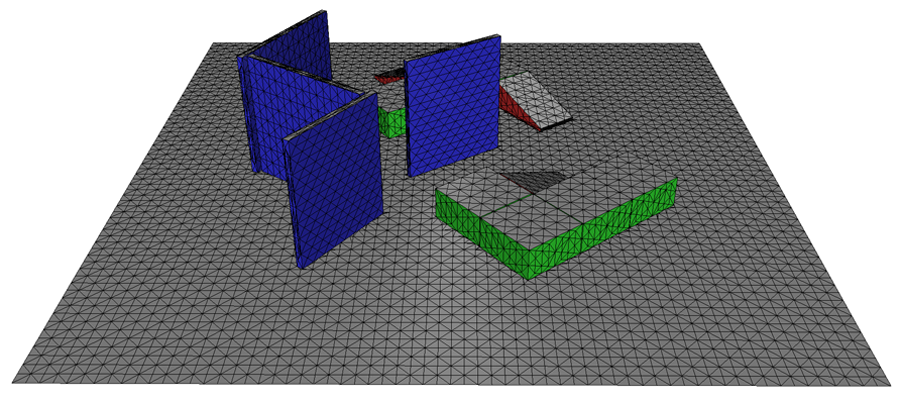
\includegraphics{images/angle2_materials.png}}\\
% \resizebox{\picwidth}{!}{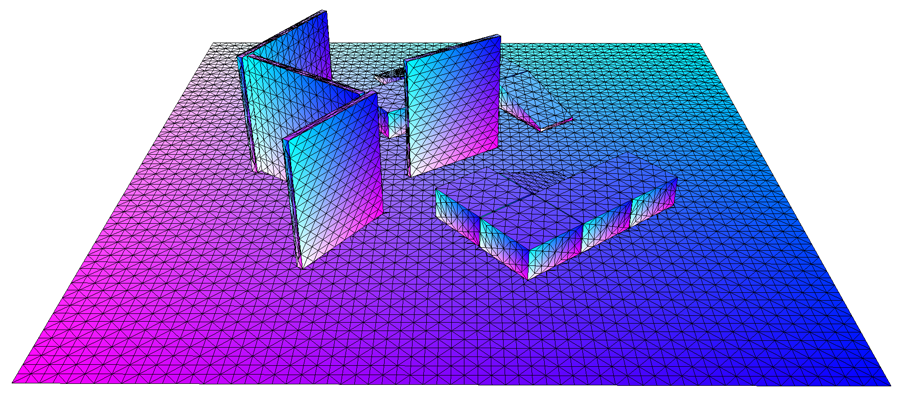
\includegraphics{images/angle2_texture_coordinates.png}}
% \end{center}
% \caption[Assignment of Material Properties]{ The world modeling
%   component assigns material identities to the surfaces of the model
%   according to the needs of the application.  In the top image, the
%   colors represent different material identifiers.  The bottom image
%   is a visualization of the texture coordinates assigned to each
%   surface.  Notice that the top surfaces of platforms and ramps are
%   mapped with texture coordinates aligned with the floor, so that a
%   single continuous texture can be applied.  }
% \label{FIGURE:MaterialProperties}
% \end{figure*}

%The ability to apply virtual textures to specific physical objects and
%surfaces in the scene is a basic primary feature of our dynamic
%projection system.  
The positions and orientations of detected objects are used to create
a virtual representation of the scene in the form of a
three-dimensional mesh with texture coordinates for each surface.
%, which are then used by applications to specify textures
%for display.  In other words, applications use the projection system
%to augment objects by assigning textures to each of the identified
%surfaces.
%(Figure~\ref{FIGURE:MaterialProperties}).
The ARmy application displays information on the horizontal surfaces
through a single overlay texture, which is shared by the table surface
and the top surfaces of all platforms and ramps.  The overlay is of
the same resolution as the 512$\times$512 heightfield, such that each
pixel corresponds directly to a single position in the game world.
Although this resolution is sufficient for covering the 42'' diameter
table, higher resolutions would improve the quality of the
visualizations and game play, allowing for smoother textures and more
detailed display icons.


\section{User Study}

We had several goals in designing the user study for our
spatially augmented gaming prototype.  The first goal was to
determine if interaction with the system was natural and intuitive and
to judge the learning curve for users familiar with games and
computers but new to spatially augmented reality.  A companion goal
was to assess the stability and robustness of our spatially augmented
reality system under heavy use by non-developers of the system.  Most
importantly, we wanted to solicit feedback on the visualization
elements and overall game play.

We hypothesized that the augmented version would be less tedious, less
ambiguous or contentious, and that movement and combat would be faster.
Altogether, this would allow users to play faster through more
rounds of movement and combat, and would allow them to experiment with and
evaluate different strategies.  We also hypothesized that users
would find the augmented reality technology more fun and immersive
than the low tech version of the game.


\subsection{Study Design}

To have a fair comparison, we designed the study as a direct
comparison of the same basic game played two different ways: using
traditional non-augmented technology (rulers \& dice), and using
the projector augmentation.  We held constant the game rules, including the
turn sequence, movement restrictions, combat sight lines, and combat
probabilities.

After an introduction to the SAR system and a brief description of the
games rules (~10 minutes), the participants played the
game three times.  The preliminary game was a short practice round
(~15 minutes) in which the participants were instructed
to use {\em both} the traditional mechanisms of rulers and dice and
the projected visualizations of movement areas and combat circles.  In
the practice round each player started with 5 army units and we
encouraged the participants to set up near their opponent to ensure
they gained experience with the combat rules.  Most participants
played 1 or 2 full cycles of game play (movement for each player and
joint combat after each movement phase) to familiarize themselves with
the rules.

Next the participants played two full games, one with and one without
augmentation, in randomly-selected order.  For each of the full games, players started with 12 units each and played for a maximum of 20
minutes.  Participants were specifically {\em not allowed} to use
rulers and dice when playing the augmented game.  Similarly, all
projector visualization and texturing was disabled for the
non-augmented version.

The supplementary video shows sample footage of both the augmented and
non-augmented versions of the movement and battle phases of the game.  
The script (read aloud to
participants) for the user study is included as supplementary
material.

\subsection{Participants}

We recruited students from the Games and Simulation Arts and Sciences
undergraduate major, which consists of artists and computer scientists
(and dual majors).
%
We believe it is important to find participants who enjoy playing
games and have a sense of competitiveness, strategy, and intellectual
curiosity when doing so.
%
We had a range of participants from freshmen through graduate
students.  In total, 26 users participated in the initial pilot study
(3 females, 5 males) or the main study (6 females, 12 males).  We made
a few revisions to the instructions and questionnaire after the pilot
study, but the procedure and data collected was quite similar between
the two studies.  We summarize the background for the participants in
the main study: 13 of the 18 participants are studying game design
with 0.5-5 years formal education in game studies.  12 of the
participants have at least 3 years formal education in computer
science.  11 of the participants have had at least 1 year of formal
art education, 7 have had at least 4 years art education.  All users
had at least 3 years experience playing computer games, 14 had more
than 10 years experience.  All users had experience playing board
games, 15 of them had more than 10 years experience.  Half of the
users had prior experience (0.5-3 years) with table top games similar
to {\em Warhammer 40,000}.  The varied pool of users provided us
with a valuable range of feedback from the study. 
%\fbox{wording... last sentence necessary?}

\subsection{Targeting polls from Written Questionnaire}


At the end of all game play, each user filled out a questionnaire.
The written questionnaire is included as supplementary material.  We
asked users to directly compare the augmented and non-augmented
versions of the game by rating on a scale of 1 to 5 each of the
following characteristics of the game:\vspace{-0.1in}

\begin{itemize}

\item the accuracy of distance calculations \\(1=inaccurate, 5=accurate)\vspace{-0.1in}
\item the accuracy of line of sight calculations for combat \\(1=inaccurate, 5=accurate)\vspace{-0.1in}
\item the accuracy of game rule implementation \\(1=frequent errors or confusion, 5=no errors or confusion)\vspace{-0.1in}
\item the subjectivity of enforcement of the rules \\(1=subjective/some disagreement, 5=no disagreement)\vspace{-0.1in}
\item their interest level during game play \\(1=tedious or boring, 5=engaging and fun)\vspace{-0.1in}

\end{itemize}

\begin{table}[tb]
\begin{center}
\begin{tabular}{@{}l|c@{~}c|c@{~}c|c@{}}
                & \multicolumn{2}{c|}{non-augmented} & \multicolumn{2}{c|}{augmented} & $\Delta$ \\
avg. rating     & all(18) & 2$^{nd}$only(10) & all(18) & 2$^{nd}$only(8) & all \\ \hline
acc. distance   & 3.6 & 4.0 & 4.5 & 4.1 & 0.8 \\
acc. sightlines & 3.8 & 4.0 & 4.8 & 4.6 & 0.9 \\
acc. rules      & 3.9 & 3.9 & 4.6 & 4.4 & 0.8 \\
subjectivity    & 4.0 & 3.9 & 4.6 & 4.6 & 0.6 \\
interest        & 3.5 & 3.9 & 4.6 & 4.6 & 1.1 \\
\end{tabular}
\end{center}%
\vspace{-0.15in}
\caption{Participant's rating of the accuracy of distance
  calculations, line-of-sight judgements, and implementation of rules,
  their assessment of the subjectivity of rule enforcement, and their
  overall interest while playing the game.  Each is scored on a scale
  of 1 to 5, with 5 being the positive attribute quality.
\label{table:timing_questionnaire}
\vspace{-0.1in}
}
\end{table}


The results of these ratings are summarized in
Table~\ref{table:timing_questionnaire}.  The average rating for all
18 study participants for each version of the game is provided.  We
also separately average the ratings of the users who played that
version of the game as their \emph{second} playthrough (when they were more familiar with the game
mechanics, rules, and strategy).  8 participants (4 pairs) played the
non-augmented version first.  10 participants (5 pairs) played the
augmented version first.

Overall, the ratings indicate that participants were interested in
playing both games, thought that the different game mechanics
were generally accurate, found enforcement of rules was not too
subjective, felt that the game was fair, and rarely
disagreed with each other or with the computer.  The
participants did consistently rate the
augmented version of the system more positively on each
characteristic. 


\subsection{Timing Results}

We used a video camera to record the experiments, which allowed us to
review the timing data for each game.  We measured the time for
terrain setup, the time for initial army placement, the average time
for each player's movement phase (red or green), the average time for
a combat round, and the average time for a battle (when two units
face off, requiring each player to roll once).  We also counted the
number of rounds (red move/combat/green move/combat) per game, and the
number of battles per game. 
%\fbox{ Is there a better way to explain what a round is?}
A summary of this data is presented in
Table~\ref{table:timing_stats}.  The timing data allows us to compare
the efficiency or speed of game play with and without augmentation.
We present the data averaged over all experiments and a separate
average of the full games that were played as the {\em second} full playthrough, when players
are most familiar with the game rules and strategy.  Note: Due to
video errors, a few of the game recordings are incomplete and are thus
omitted from these averages.

Game setup is slower with the augmented system for both terrain layout
(100\% slower) and army unit placement (10\% slower).  This is due to
a number of minor factors: triggering the remote, waiting for the
visualization system to refresh, and reminding players to remove all
unnecessary materials from the game table and step out of the
camera's field of view.  Similarly, movement phases are 25\% slower
in the augmented version.  We note that in the augmented version,
because moves are validated by the system, extra time is required when
players must correct illegal moves.  With system overhead optimization
we believe these differences can be greatly reduced.  In particular, we
believe these improvements combined with user familiarity with the movement
region visualization will allow movement phases to be
faster in the augmented version than in the non-augmented version.

\begin{table}[tb]
\begin{center}
\begin{tabular}{@{}l|cc|cc@{}}
               & \multicolumn{2}{c|}{non-augmented} & \multicolumn{2}{c}{augmented} \\
averages       & all(9) & 2$^{nd}$only(3) & all(9) & 2$^{nd}$only(5) \\ \hline
terrain setup  & 1:16    & 1:13         & 2:46    & 2:07         \\
army placement & 2:52    & 2:38         & 3:03    & 3:11 \\ 
movement phase & 0:42    & 0:36         & 0:52    & 0:47 \\
combat phase   & 1:33    & 2:13         & 0:22    & 0:18 \\
single battle  & 0:16    & 0:21         & 0:04    & 0:03 \\ \hline
\# rounds per game & 2.3  & 2.0         & 3.9     & 4.1 \\
\# battles per game & 26.1   & 24.5   &  36.6    & 41.0 
\end{tabular}
\end{center}%
\vspace{-0.15in}
\caption{ The average timing data (minutes:seconds) for various stages
  of game play are summarized for both non-augmented (traditional) and
  SAR augmented experiments.
\label{table:timing_stats}
}
\vspace{-0.1in}
\end{table}

Not-surprisingly, the augmented system's main efficiency improvement
is gained in the combat simulation phase (roughly 4X faster).  The result of each
separate battle is visualized one-at-a-time for the
players (approximately 1 
%\fbox{???}  
second per virtual ``die'' roll),
which is faster than humans typically roll dice.  Note that the combat
phase also includes removal of disabled units at the end of the phase.
However, the greatest efficiency improvement is in calculating which
units have line of sight and are in range, and {\em most importantly},
in keeping track of which battles have occurred and correctly
accounting for all combinations of opposing units when they are
densely clustered.

As we hypothesized, overall the augmented version allows players to
complete more cycles of game play before time is called (60\% more),
and similarly, more total battles are fought (40\% more) in the
augmented version.


\subsection{Verbal and Written Feedback}

We encouraged the participants to talk aloud to each other and the
experimenters, offering feedback and asking questions throughout the
study.  Each participant also answered several short answer questions
on the written form giving us further insight about the positive and
negative aspects of each game mode.  Overall two participants
preferred the non-augmented game, fifteen preferred the augmented
version, and one person called it a tie.  Many participants had the
same general comments about the games.  A summary of these comments:

\newcommand{\mysep}{-0.08in}

%\begin{small}
\paragraph{Positive Aspects of Traditional, Non-Augmented Game:}

\begin{itemize}

\vspace{-0.05in}

\item 
%felt like traditional board game
``It was a little more hands on'' and
``player decisions were more fluid'', which
``keeps players actively involved in game play''.\vspace{\mysep}

\item 
Tactile control allowed participants to ``know exact outcome of dice''
and they ``felt responsible for the outcome of the
dice''.\vspace{\mysep}

\item 
Users appreciated the
%wiggle room in interpretation of the ryles
``slight bending of rules for more realistic and entertaining game play''.
%it was easier to do certain things, like skip a turn or make mutal agreements on rulings or confusion


%being able to check whether you were in range without waiting for the system to update
%not having to worry about glitches

\end{itemize}

\paragraph{Negative Aspects of Traditional, Non-Augmented Game:}

\begin{itemize}

\vspace{-0.05in}

\item 
%time consuming
%measuring is tedious
``Much slower combat (actually rolling the dice each time and making sure every combination of soldiers is accounted for)''
%dice kept falling off table 
and
``when many attacks [happened] at the same time, it made the game stop and not be fun''.
\vspace{\mysep}

\item 
%difficult to keep up with everything during combat
``In a dense soldier cluster there were so many attacks made that we probably lost count at some point and either attacked too many times or too few''.
%``a slightly sloppy feel where i felt that i could be making mistakes''
%sometimes it was tricky remembering which pairs of soldiers had already fired, but we came up with a strategy that mostly solved that.
Most participants experienced ``occasional confusion (even about whose turn it was)''.%
\vspace{\mysep}

\item 
%some subjectivity with measurements
Subjectivity: ``While we made decisions, they were not necessarily the
correct ones in terms of the rules''.

\end{itemize}

\paragraph{Positive Aspects of Game with Projection Augmentation:}


\begin{itemize}

\vspace{-0.05in}

\item
Participants found that the ``visualizations were easy to understand'',
it was
%can see where you're going
``easy to see how far you can move'',
%distances were clearly marked as well as line of sight and current shooting pairs.
and it was ``never unclear about whose turn it was or what could be done''.
%``no questioning who was on higher ground''
\vspace{\mysep}

\item 
%didn't have to do any work
Most participants ``trust [the] computer'' and the games had
``no disagreement between players since there was an ultimate referee''.
%no human errors
%it fixed the "wait did he shoot yet?" problem.  
\vspace{\mysep}

\item 
%projected scenery made me feel like i was playing a game and not a probability simulator
%visually it was far more interesting
The use of projective texture was  ``more visually stimulating''
and the animations of
``the arrows for combat were amusing to watch''.
\vspace{\mysep}

\item 
Several participants specifically commented that faster, more
efficient play made it ``much easier to establish movement strategy''
%combat was faster
%considerably quicker pace
because ``it allowed you to focus on the game play and not the math
behind it''.

\end{itemize}

\noindent
\paragraph{Negative Aspects of Game with Projection Augmentation:}



\begin{itemize}

\vspace{-0.05in}
\item ``Turns were slow'' while ``waiting for recalculation'' and
  ``moving pieces slightly out of range made it take longer
  sometimes''. \vspace{\mysep}

%switching between turns was a little slow.

\item
Occasional system glitches and the ``restriction in terrain placement because of projection'' were negatives.
% (vision)
%minor issues identifying scenery
%some setup bugs
%occasional glitches
%things not getting detected for being in certain positions
%wall blockage issue with camera, couldn't move too close to walls.
``Blind spots forced us to simplify our first terrain design a bit,
but that's a natural consequence of using a single camera''.
\vspace{\mysep}

\item
Explanation of game results was sometimes unclear: 
``Don't know the reason the soldier was disabled''.
\vspace{\mysep}

\item
``Took the player engagement away a bit.  Watched action happen rather
than rolling the dice.  Takes away your feeling of involvement.''
%hard to see line of sight sometimes

%some rules implemented questionable
\end{itemize}

%\end{small}




%%%%%%%%%%%%%%%%%




\section{Conclusions and Future Work}
%\fbox{I put the negative first}

Our SAR system could benefit from several specific improvements, many
of which point to interesting avenues of future research.  One
significant improvement would be to incorporate a method for
simultaneous acquisition and display, allowing for the system to react
to users in realtime, without the need for turn-based update requests.
A more sophisticated tracking scheme could also lead to improved
object identification. Additional means for user interaction, such as
gesture-based or verbal speech controls, could also be beneficial.
Finally, play could be enhanced by displaying some state information
directly onto the units themselves to remove clutter, and by adding
audio elements to increase the immersive feel of the game.

Overall, the ARmy application is a fully functional prototype that
demonstrates the key benefits of spatially augmented reality and shows
how a tangible tabletop interface can be combined with a video game
module to create an entertaining user experience.  The results of our
user study indicate a general participant preference for the augmented
version of our game prototype, and feedback has shown a positive
opinion about SAR technology in the context of tabletop
games. 
%\fbox{meh...}

%% \paragraph{Simultaneous Acquisition and Display}

%% As previously explained, our small-scale tabletop system is currently %% incapable of simultaneous acquisition and display.  Although this has %% not prevented development of interesting applications that update upon %% user command, such as the turn-based ARmy game, feedback from %% potential users after an informational demonstration of the prototype %% indicates that these applications might be more appealing if the %% system updated automatically in real-time.  %\fbox{Why?}

%% Accomplishing this would require overcoming a number of challenges.  %% The primary issue is that our current color-based object tracking %% methods are not robust enough to ignore the influence of the projected %% visuals.  One possible solution would be to use infrared marker-based %% detection as we do in the large-scale case, but this would add the %% requirement of attaching suitable markers to all display objects, %% which is impractical in the cases of small, detailed objects, such as %% the plastic soldier figurines.  A more promising idea would be to %% leverage more precise synchronization between the camera and %% projectors in order to interleave periods of acquisition and periods %% of display at imperceptibly fast speeds.

%% Yet another possibility would be to abandon color-based and %% marker-based techniques altogether, in favor of structured light %% techniques.  In this case, imperceptible pattern embedding techniques %% or infrared light techniques could provide a sensible solution.  These %% changes would likely also require a shift in paradigm of how specific %% objects are recognized in order to use the depth information that %% these methods provide, perhaps adopting a technique similar to the %% pose-estimation employed by the Kinect~\cite{Kinect, Shotton2011}.  %% Ultimately, this could lead to more robust tracking of a larger, more %% flexible collection of objects.  For example, more unique terrain with %% complex variations in elevation could be used in place of the %% relatively primitive platforms and ramps of the current application.

%% Users interacting with objects on the table are likely to occlude %% parts of the table from the camera, thereby presenting another hurdle %% to real-time acquisition.  At present, users are instructed to step %% back from the table before requesting an update to ensure that such %% occlusions do not occur.  One way to handle this problem would be to %% implement an algorithm for detecting when occlusions have occurred and %% to simply update only objects that are visible to the camera.  %% Incorporating additional cameras would also improve the situation by %% allowing objects to be detected from multiple points of view.

%% \subsection{Improvements to Object Identification }

%% Because the system currently lacks the ability to distinguish between %% objects with similar shape and color properties, it is relatively %% common for object identities to be accidentally swapped.  Improved %% object recognition could allow for unique identification of each %% object, instead of relying solely on frame-to-frame temporal %% coherence.  In the case of the ARmy application, this would allow for %% more complex game mechanics, such as the introduction of multiple %% types of unique units.  Ideally, for this technology to be applied to %% an existing commercial tabletop game, the tracking module would need %% to be able to reliably identify units from the large library of %% available miniatures, including ones that may have been painted or %% otherwise customized by players.

%% The current ARmy application uses the projector system for overlaying %% information and visually augmenting only the terrain objects.  More %% accurate representation of figurine models could allow for increased %% opportunities for direct augmentation.  Instead of simply augmenting %% the terrain, we could paint elements directly onto figurine surfaces, %% again allowing users to integrate undecorated game pieces and highly %% detailed ones without compromising aesthetic quality.  Additionally, %% displaying state information onto the units themselves could reduce %% the amount of visual clutter that must be overlaid onto the table %% surface.

%% \subsection{Additional User Interactions }

%% Perhaps the most significant way in which the user interface of our %% tabletop system could be expanded would be to provide the user with %% additional means of interacting with objects other than by physically %% moving them.  Ideally, users should be able to ``select'' objects by %% pointing or otherwise gesturing.  For example, the ARmy application %% would greatly benefit by allowing users to toggle the information %% display of specific units and to explicitly designate targets during %% combat rounds.

%% An obvious first step in solving this problem would be to integrate %% our infrared laser pointing techniques within our small-scale system.  %% However, a preferable solution would not require users to interact %% through extraneous devices, but to instead use physical gestures, such %% as pointing with their hands.  In addition to picking objects, %% hand-tracking methods could facilitate other user interactions, %% replacing the wireless remote used by many of our applications.  

%% The benefits of user tracking are not limited to our small-scale %% applications.  Positional data of users moving through our large-scale %% display environment could be used to automatically focus and expand %% visual information as appropriate.  A potential first step for our %% system would be to provide users with wearable markers detectable by %% our infrared camera module.  Ideally however, we would be able to track %% users without the need for such markers, which might interfere with %% the user's comfort and mobility.  Additionally, more complex body %% tracking could allow for gestural controls.

%Currently, out system computes a set of projector blending weights %for each vertex of the scene geometry in order to achieve a sense of %seamlessness in the multiprojector display.  However, this component %could be improved by adopting a more accurate per-pixel method using %depth buffer techniques similar to shadow maps.  A further step would %be to integrate this techniques with some method of color correction, %in order to reduce the variation of color information between %projectors.

%% \subsection{Audio Features}

%% Our research up to this point has almost completely ignored the %% prospect of adding audio output to our applications, a feature that %% could be especially useful in our large-scale system, which ultimately %% aims for an increased sense of immersion.  Although a few of our %% applications have featured audio elements, such as the ping pong %% application's sound effects, we have not yet explored any output %% device configurations beyond using a single speaker.  Since our system %% is centered on the ability of the users to change the display setup at %% will, optimal integration of audio elements into a dynamic scene %% presents an interesting problem with a number of challenges.  In the %% future, our research group looks forward to opportunities to work with %% acoustic specialists in this regard.  Audio input offers another %% interesting set of possibilities.  For example, voice-activated %% commands could be used in combination with the existing user input %% methods to produce an even better, more natural interface.

%\fbox{end with paragraph about ubiquity of tech? }



%\section{Conclusion}


%\fbox{WRITE THIS}
%% if specified like this the section will be omitted in review mode
%\acknowledgements{
%The authors wish to thank A, B, C. This work was supported in part by
%a grant from XYZ.}

\bibliographystyle{abbrv}
%%use following if all content of bibtex file should be shown
%\nocite{*}
\bibliography{thesis}
\end{document}
